
\section{三维图类型}
\label{sec:3d}

{
\tikzset{external/figure name/.add={}{threedim_}}

\PGFPlots{} 提供三维可视化，如散点图、线图、网格图或曲面图。本节解释
提供输入坐标的方法以及如何使用不同的图类型。


\subsection{开始使用 3D 之前}

在深入探讨 \PGFPlots{} 的三维可视化功能之前，让我先从一些预备说明
开始。将 \PGFPlots{} 用于三维图的原因与普通二维图的原因类似：可以
获得一致的字体和文档一致的样式，同时输出高质量。

虽然这对于（不太复杂的）二维图效果很好，但它比非图形文档需要相当多的
精力。对于三维图更是如此。换句话说：\PGFPlots{} 的三维例程很慢。
这其中有原因，其中一些可能在未来版本中消失。但其中一个原因是 \TeX{}
从未为复杂的可视化技术而设计。考虑使用 |lualatex|（以及至少
|compat=1.12|）以减少编译时间并避免内存限制。另外请考虑
\ref{sec:pgfplots:export} 节中提到的图像例程化例程，特别是 |external|
库，以减少排版时间。除了速度限制外，三维图很容易达到内存限制。因此，
三维图的图复杂度被限制在相对粗略的分辨率。\ref{sec:pgfplots:export}
节还讨论了扩展初始 \TeX{} 内存限制的方法。

三维可视化中出现的另一个问题是深度：需要决定哪些项要绘制在其他项
前面。\PGFPlots{} 在一定程度上支持 $z$ 缓冲技术：它对于单个散点图
（|z buffer=sort|）、网格或曲面图（|z buffer=auto|）或参数网格和曲面
图（|z buffer=sort|）效果很好。但是，它不能组合不同的
|\addplot| 命令，这些命令将按出现顺序绘制。你有时可能会遇到这些限制。
也许在未来版本中会改进。

如果你决定需要高复杂度、速度和 100\% 可靠的 z 缓冲（深度信息），
你应该考虑使用其他可视化工具，几年后再回到 \PGFPlots{}。如果你可以
等待复杂图片，甚至看不到 z 缓冲限制带来的局限性，你应该使用
\PGFPlots{}。再次提醒，考虑使用 |external| 库的自动图片例程化，
如 \ref{sec:pgfplots:export} 节所讨论。


\subsection{\texttt{\textbackslash addplot3} 命令：三维坐标输入}
\label{sec:pgfplots:sec:threedim}

\begin{addplot3generic}
    \verbpdfref{\addplot3} 命令是任何三维图的主要接口。它的工作方式与
    其二维变体 |\addplot| 相同，后者在第\pageref{sec:addplot}页的
    \ref{sec:addplot} 节中详细描述。

    \verbpdfref{\addplot3} 命令接受与 |\addplot| 变体相同的输入方法，
    包括表达式绘图、坐标、文件和表。但是，这些方法中的每一种都需要
    第三个坐标，这通常是直接的，并在下面详细解释。

    此外，\verbpdfref{\addplot3} 有一种方法来决定是要进行\emph{线}
    可视化还是\emph{网格}可视化\index{3d: line or mesh}。前者是从
    一维到 $\R^3$ 的映射，后者是从二维到 $\R^3$ 的映射。这里，键
    |mesh/rows| 和 |mesh/cols| 用于定义网格大小（矩阵大小）。通常，
    你不需要关心这个，因为坐标输入例程已经允许一维或二维结构。

    \PGFPlots{} 区分线可视化和网格可视化的精确规则如下：
    %
    \begin{enumerate}
        \item 如果已使用键 |mesh input=patches|，\PGFPlots{} 依赖于
            当前的 |patch type|（它具有固有维度）。
        \item 对于 |mesh input| 的所有其他值（如 |mesh input=lattice|
            和 |mesh input=image|），\PGFPlots{} 按以下方式处理：
            %
            \begin{itemize}
                \item 它自动补全 |mesh/rows| 和 |mesh/cols| 的值
                    （或使用它们的规定值）。
                \item 如果这些键描述大小为 $1\times N$ 或
                    $N \times 1$ 的矩阵，\PGFPlots{} 假设它是一条线。
            \end{itemize}

            "自动补全"取决于你如何提供数据。
            %
            \begin{itemize}
                \item 如果你使用 \verbpdfref{\addplot3 expression}，
                    |mesh/rows| 和 |mesh/cols| 从值 |samples| 和
                    |samples y| 计算。默认情况下，
                    \verbpdfref{\addplot3 expression} 始终对网格采样。
                    如果你希望它对一条线采样，设置 |samples y=1|
                    （或等价地，|y domain=0:0|）。
                \item 如果你使用 \verbpdfref{\addplot3 table}、
                    \verbpdfref{\addplot3 coordinates} 或
                    \verbpdfref{\addplot3 file}，你基本上有两个选择：
                    要么显式提供 |mesh/rows| 或 |mesh/cols| 中的至少
                    一个，要么通过扫描线结束标记格式化输入表，如
                    |empty line=auto| 或 |empty line=scanline| 中所述。
                    在这种情况下，\PGFPlots{} 计算扫描线长度并使用
                    |mesh/ordering| 来推断如何确定矩阵值。

                    因此，如果你的输入表中有空行，\PGFPlots{} 将自动
                    识别矩阵大小。

                    如果你\emph{没有}空行，\PGFPlots{} 期望
                    |mesh/rows| 或 |mesh/cols| 中的至少一个。
            \end{itemize}
    \end{enumerate}
\end{addplot3generic}

\begin{addplot3operation}[]{coordinates}{\marg{coordinate list}}
    \verbpdfref{\addplot3 coordinates} 方法的工作方式与其二维变体
    \verbpdfref{\addplot coordinates} 相同，后者在第
    \pageref{pgfplots:addplot:coordinates} 页详细描述：

    预期有一个长坐标列表 |(|\meta{x}|,|\meta{y}|,|\meta{z}|)|，以空白
    分隔。输入列表可以是坐标的无序序列，例如用于散点图或线图。它也
    可以具有矩阵结构，在这种情况下，一个 |empty line|（等同于
    "|\par|"）标记一个矩阵行的结束。如果显式提供 |mesh/rows| 或
    |mesh/cols| 中的一个，也可以提供矩阵结构。

\begin{codeexample}[]
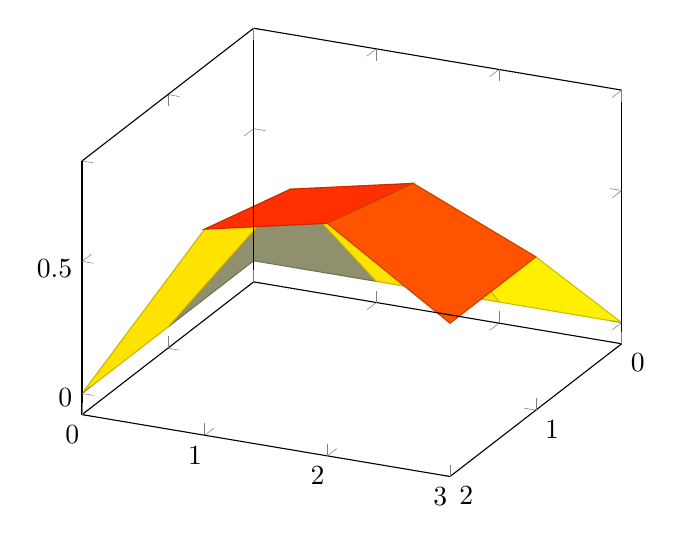
\begin{tikzpicture}
\begin{axis}
    % this yields a 3x4 matrix:
    \addplot3 [surf] coordinates {
        (0,0,0) (1,0,0)   (2,0,0)   (3,0,0)

        (0,1,0) (1,1,0.6) (2,1,0.7) (3,1,0.5)

        (0,2,0) (1,2,0.7) (2,2,0.8) (3,2,0.5)
    };
\end{axis}
\end{tikzpicture}
\end{codeexample}
    %
    \noindent 这里，\verbpdfref{\addplot3} 读取一个三行四列的矩阵。
    |empty line| 将一行与下一行分开。

    对于二维 |\addplot coordinates|，可以在单个坐标内提供（常量）
    数学表达式。语法 |(|\meta{x}|,|\meta{y}|,|\meta{z}|) |\oarg{meta}
    可以像二维 |\addplot coordinates| 一样用于提供显式颜色数据；
    误差棒也受支持。
\end{addplot3operation}

\begin{addplot3operation}[]{table}{\oarg{column selection}\marg{file}}
    \verbpdfref{\addplot3 table} 输入的工作方式与其二维对应物
    \verbpdfref{\addplot table} 相同。它仅期望 $z$ 坐标的一列。

    与 \verbpdfref{\addplot3 coordinates} 一样，文件中的一个
    |empty line| 标记一个矩阵行的结束。

    对于文件中的矩阵数据，重要的是指定矩阵条目的写入顺序。默认
    配置是 |mesh/ordering=x varies|，因此如果你有逐列顺序，则需要
    将其更改为 |mesh/ordering=y varies|。

\begin{codeexample}[]
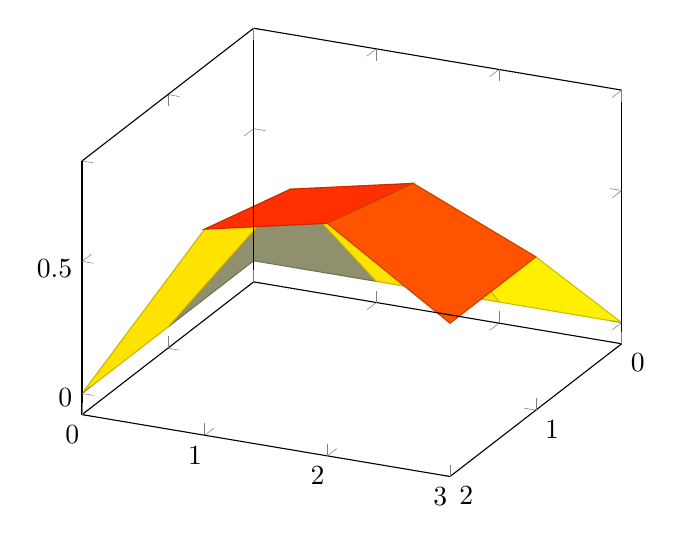
\begin{tikzpicture}
\begin{axis}
    % this yields a 3x4 matrix:
    \addplot3 [surf] table {
         0 0 0
         1 0 0
         2 0 0
         3 0 0

         0 1 0
         1 1 0.6
         2 1 0.7
         3 1 0.5

         0 2 0
         1 2 0.7
         2 2 0.8
         3 2 0.5
    };
\end{axis}
\end{tikzpicture}
\end{codeexample}
\end{addplot3operation}

\begin{addplot3operation}[]{file}{\marg{name}}
    \paragraph{弃用说明：}

    如果你有数据文件，通常应该使用 |\addplot table|。输入类型
    |\addplot file| 几乎相同，但功能要弱得多。它仅为向后兼容而保留。

    \verbpdfref{\addplot3 file} 输入方法与 \verbpdfref{\addplot file}
    相同——它仅多期望一个坐标。因此，输入文件在第一列包含 $x_i$，
    第二列包含 $y_i$，第三列包含 $z_i$。

    如果请求了 |point meta=explicit|，则在 $z_i$ 之后读取另一列，
    详情参见第\pageref{pgfplots:addplot:file}页的
    \verbpdfref{\addplot file} 文档。

    与 \verbpdfref{\addplot3 coordinates} 一样，文件中的一个
    |empty line| 标记一个矩阵行的结束。
    %
\begin{codeexample}[]
\begin{tikzpicture}
\begin{axis}
    % We have `plotdata/first3d.dat' with
    %---------
    % 0 0 0.8
    % 1 0 0.56
    % 2 0 0.5
    % 3 0 0.75
    %
    % 0 1 0.6
    % 1 1 0.3
    % 2 1 0.21
    % 3 1 0.3
    %
    % 0 2 0.68
    % 1 2 0.22
    % 2 2 0.25
    % 3 2 0.4
    %
    % 0 3 0.7
    % 1 3 0.5
    % 2 3 0.58
    % 3 3 0.9
    % -> yields a 4x4 matrix:
    \addplot3 [surf] file {plotdata/first3d.dat};
\end{axis}
\end{tikzpicture}
\end{codeexample}

    对于文件中的矩阵数据，重要的是指定矩阵条目的写入顺序。默认
    配置是 |mesh/ordering=x varies|，因此如果你的矩阵是按列顺序存储的，需要将其更改为
    |mesh/ordering=y varies|。
\end{addplot3operation}

\begin{pgfplotskeylist}{mesh/rows=\marg{integer},mesh/cols=\marg{integer}}
    对于需要某种矩阵输入的网格或曲面图的可视化，需要知道输入矩阵
    的维度才能正确可视化图形。矩阵结构可能从行结束标记（输入流中
    作为通用扫描线结束标记的 |empty line|）获知，如上所述。

    如果矩阵结构尚不知道，需要提供 |mesh/rows| 或 |mesh/cols|
    之一，其中 |mesh/rows| 表示 $y$ 坐标的样本数，而 |mesh/cols|
    是用于 $x$ 坐标的样本数（另见 |mesh/ordering|）。

    因此，以下示例也是定义输入矩阵的有效方法。
    %
\begin{codeexample}[]
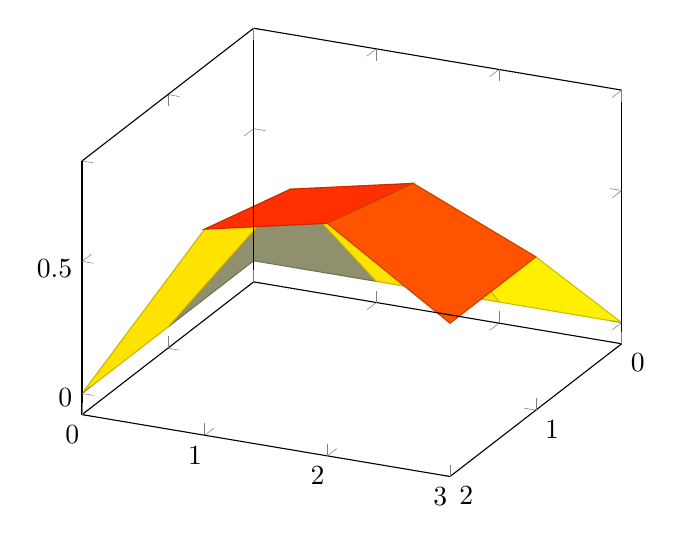
\begin{tikzpicture}
\begin{axis}
    % this yields also a 3x4 matrix:
    \addplot3 [surf,mesh/rows=3] coordinates {
        (0,0,0) (1,0,0)   (2,0,0)   (3,0,0)
        (0,1,0) (1,1,0.6) (2,1,0.7) (3,1,0.5)
        (0,2,0) (1,2,0.7) (2,2,0.8) (3,2,0.5)
    };
\end{axis}
\end{tikzpicture}
\end{codeexample}
    只需提供 |mesh/rows| 或 |mesh/cols| 中的一个——缺失的值将自动确定。

    如果你提供 |mesh/rows| 或 |mesh/cols| 中的一个，输入文件或坐标流
    中看到的任何行结束标记都将被忽略。
\end{pgfplotskeylist}

\begin{pgfplotskeylist}{mesh/scanline verbose=\mchoice{true,false} (initially false)}
    在 \LaTeX{} 输出中提供关于扫描线结束标记的调试消息。

    该消息将告知是否找到了扫描线结束标记以及它们是否相同。
\end{pgfplotskeylist}

\begin{pgfplotskey}{mesh/ordering=\mchoice{x varies,y varies,rowwise,colwise} (initially x varies)}
    允许配置从 \verbpdfref{\addplot3 coordinates}、
    \verbpdfref{\addplot3 file} 或 \verbpdfref{\addplot3 table} 读取矩阵
    （网格）的顺序。

    这里，\declaretext{x varies} 表示一个点序列，其中 $n$=|mesh/cols|
    个连续点具有固定的 $y$ 坐标。当你写下函数时这是直观的，因为 $x$
    是水平的，$y$ 是垂直的。注意，在矩阵术语中，$x$ 指\emph{列索引}，
    而 $y$ 指\emph{行索引}。因此，从这个意义上说，|x varies| 等同于
    \declaretext{rowwise} 顺序。这是初始配置。

\begin{codeexample}[]
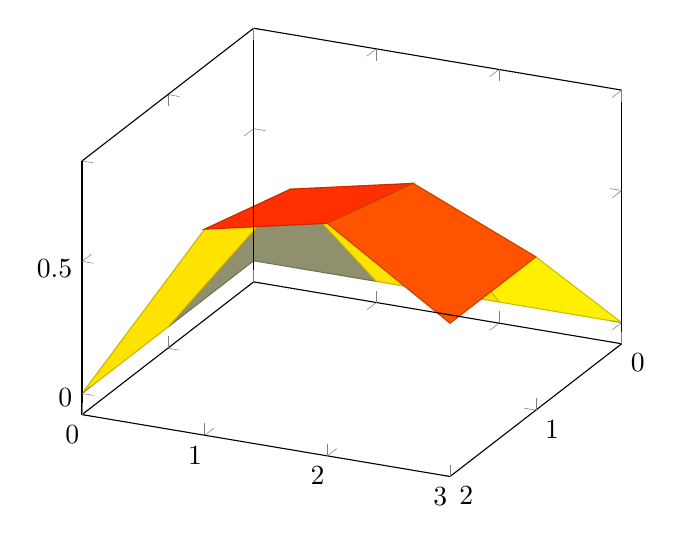
\begin{tikzpicture}
\begin{axis}[mesh/ordering=x varies]
    % this yields a 3x4 matrix in `x varies'
    % ordering:
    \addplot3 [surf] coordinates {
        (0,0,0) (1,0,0)   (2,0,0)   (3,0,0)

        (0,1,0) (1,1,0.6) (2,1,0.7) (3,1,0.5)

        (0,2,0) (1,2,0.7) (2,2,0.8) (3,2,0.5)
    };
\end{axis}
\end{tikzpicture}
\end{codeexample}
    %
    \noindent 注意，|mesh/ordering| 是必需的，即使矩阵的大小可以以
    不同方式提供。上面的示例使用 |empty line| 标记扫描线。也可以说
    |mesh/rows=3| 并省略 |empty line|。

    因此，|mesh/ordering=|\declaretext{y varies} 提供这样的点，使得
    连续的 $m$=|mesh/rows| 个点形成一列，即 $x$ 坐标固定而 $y$ 坐标
    变化。从这个意义上说，|y varies| 等同于 \declaretext{colwise}
    顺序，它实际上是一个矩阵转置。
    %
\begin{codeexample}[]
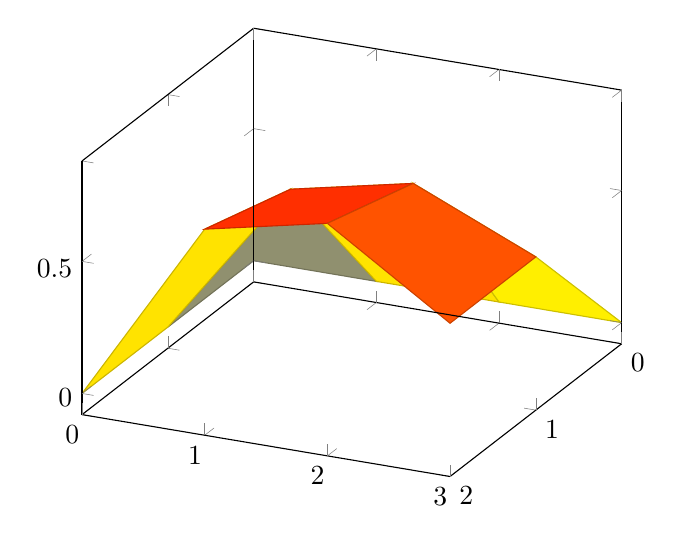
\begin{tikzpicture}
\begin{axis}[mesh/ordering=y varies]
    % this yields a 3x4 matrix in column-wise ordering:
    \addplot3 [surf] coordinates {
        (0,0,0) (0,1,0)   (0,2,0)

        (1,0,0) (1,1,0.6) (1,2,0.7)

        (2,0,0) (2,1,0.7) (2,2,0.8)

        (3,0,0) (3,1,0.5) (3,2,0.5)
    };
\end{axis}
\end{tikzpicture}
\end{codeexample}
    %
    再次注意与常见矩阵索引的微妙区别，在常见矩阵索引中一列具有固定的
    第二索引。\PGFPlots{} 指的是人们在纸上写下函数的方式（这与
    Matlab$^\text{\textregistered}$ 用矩阵显示离散函数的方式一致）。
\end{pgfplotskey}

\begin{addplot3operation}[]{\marg{math expression}}{}
\labelprefix\label{cmd:addplot3:expr}
        \pgfmanualpdflabel{\textbackslash addplot3 expression}{}%
    表达式绘图的工作方式也与二维图相同。但现在，采样的是二维网格而不是
    单条线，它可能取决于 |x| 和 |y|。

    方法 \verbpdfref{\addplot3} \marg{math expr} 可视化函数
    $f(x,y) = $\meta{math expr}，其中
    $ f \colon [x_1,x_2] \times [y_1,y_2] \to \R$。区间 $[x_1,x_2]$
    使用 |domain| 键确定，例如使用 |domain=0:1|。区间 $[y_1,y_2]$
    使用 |y domain| 键确定。如果 |y domain| 为空，则假设
    $[y_1,y_2] = [x_1,x_2]$。如果 |y domain=0:0|（或任何其他长度为
    零的区间），则假设绘图不依赖于 |y|（因此它是一个线图）。

    $x$ 方向的采样数使用 |samples| 键设置。$y$ 方向的采样数使用
    |samples y| 键设置。如果未设置 |samples y|，则使用与 $x$ 相同的
    值。如果 |samples y|$\,\le 1$，则假设绘图不依赖于 |y|
    （意味着它是一个线图）。

\pgfplotsexpensiveexample
\begin{codeexample}[]
% requires \usepgfplotslibrary{colorbrewer}
\begin{tikzpicture}
\begin{axis}[
    colormap/PuBu,
]
    \addplot3 [surf] {y};
\end{axis}
\end{tikzpicture}
\end{codeexample}

\pgfplotsexpensiveexample
\begin{codeexample}[]
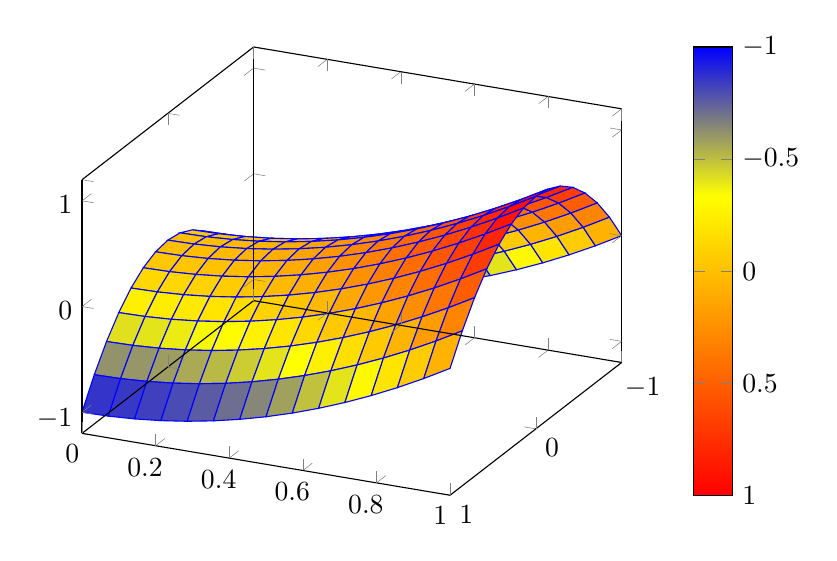
\begin{tikzpicture}
\begin{axis}[colorbar]
    \addplot3 [
        surf,
        faceted color=blue,
        samples=15,
        domain=0:1,y domain=-1:1
    ] {x^2 - y^2};
\end{axis}
\end{tikzpicture}
\end{codeexample}

    表达式绘图自动设置 |mesh/rows| 和 |mesh/cols|；这些设置对表达式
    绘图没有任何影响。
\end{addplot3operation}

\begin{addplot3operation}[]{expression}{\marg{math expression}}
    语法

    \verbpdfref{\addplot3} \marg{math expression}|;|

    是以下形式的简写等价物

    \verbpdfref{\addplot3 expression} \marg{math expression}|;|
\end{addplot3operation}

\begin{addplot3operation}[]{(\meta{$x$ expression},\meta{$y$ expression},\meta{$z$ expression})}{}
    \verbpdfref{\addplot3 expression} 的一个变体，它允许为 $x$、$y$ 和
    $z$ 坐标提供不同的坐标表达式。这可用于生成参数化图。

    请注意，|\addplot3 (x,y,x^2)| 等同于
    |\addplot3 expression {x^2}|。

    另外注意，由于完整的点表达式被圆括号包围，
    \meta{$x$ expression}、\meta{$y$ expression} 或
    \meta{$z$ expression} 内部的圆括号需要特殊处理。用花括号包围
    表达式（其中包含圆括号）：

    |\addplot3 (|\marg{$x$ expr}|, |\marg{$y$ expr}|, |\marg{$z$ expr}|);|
\end{addplot3operation}


\subsection{线图}
\label{sec:pgfplots:lineplots}

如果输入源没有矩阵结构，则生成三维线图。线图获取输入坐标并按出现顺序
连接它们。

\begin{codeexample}[]
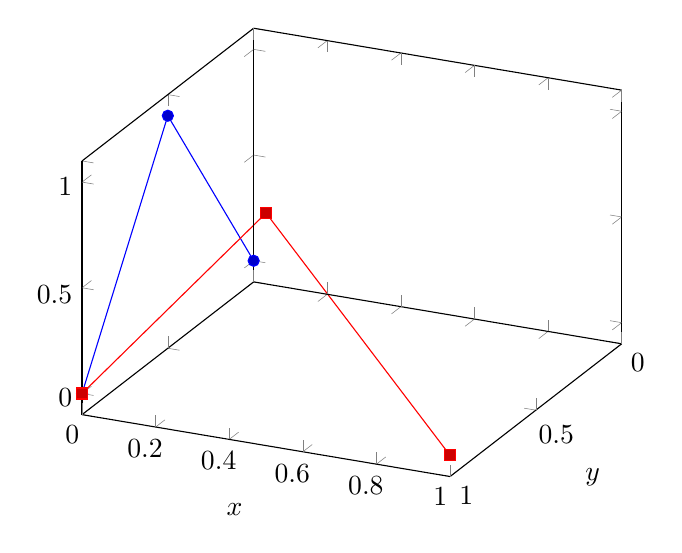
\begin{tikzpicture}
\begin{axis}[
    xlabel=$x$,
    ylabel=$y$,
]
    \addplot3 coordinates {(0,0,0) (0,0.5,1) (0,1,0)};
    \addplot3 coordinates {(0,1,0) (0.5,1,1) (1,1,0)};
\end{axis}
\end{tikzpicture}
\end{codeexample}
%
如果 |mesh/rows| 和 |mesh/cols| 都没有值，或者其中一个为 |1|，
\PGFPlots{} 将绘制线图。如果输入流中没有扫描线结束标记
（|empty line|），也是这种情况。

对于 \verbpdfref{\addplot3 expression}，这需要设置 |samples y=1|
以禁用网格的生成。
%
\begin{codeexample}[]
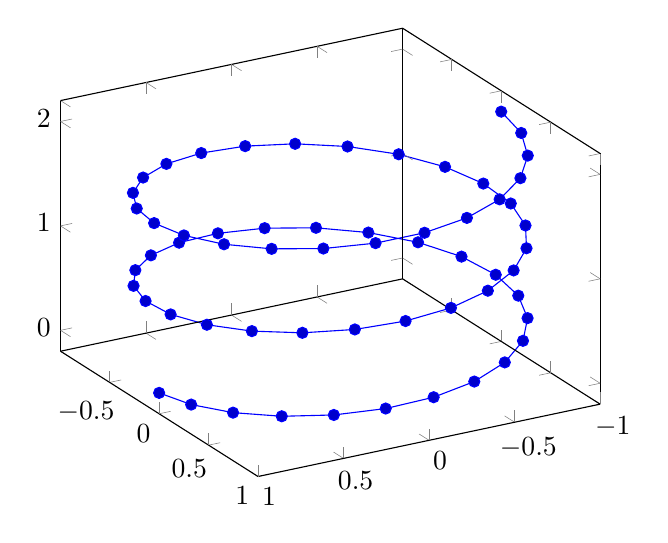
\begin{tikzpicture}
\begin{axis}[view={60}{30}]
    \addplot3+ [
        domain=0:5*pi,
        samples=60,
        samples y=0,
    ] (
        {sin(deg(x))},
        {cos(deg(x))},
        {2*x/(5*pi)}
    );
\end{axis}
\end{tikzpicture}
\end{codeexample}
%
\noindent 上面的示例是一个按表达式的参数图，即它有三个不同的表达式
用于 $x$、$y$ 和 $z$。

三维线图也可用于数据图（表）。最简单的情况是你简单地提供一系列三维
坐标，它们将按出现顺序连接：
%
\begin{codeexample}[]
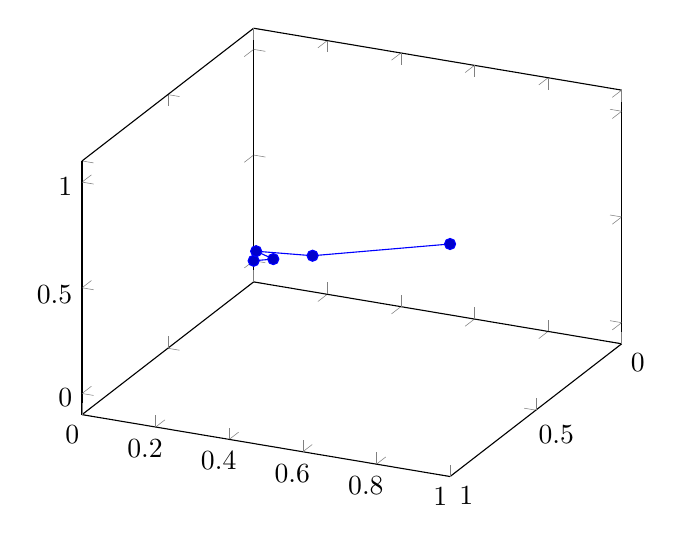
\begin{tikzpicture}
\begin{axis}
    \addplot3 table {
        x   y   z
        0   0   0
        0.1 0.1 0.1
        0.1 0.2 0.2
        0.3 0.3 0.3
        1   1   1
    };
\end{axis}
\end{tikzpicture}
\end{codeexample}
%
\noindent 注意，这个图隐式地具有 |mesh/rows=1|，因为它没有扫描线结束
标记（|empty line|）。如果不确定，可以显式设置 |mesh/rows=1| 以告诉
\PGFPlots{} 你有一维数据（而不是矩阵）。

如果数据文件仅包含两个坐标——而第三个坐标应该以某种方式提供，那么
来自数据文件的线图也是可能的。在这种情况下，|table/x expr| 功能
发挥作用：它允许组合数据图和数学表达式：
%
\begin{codeexample}[]
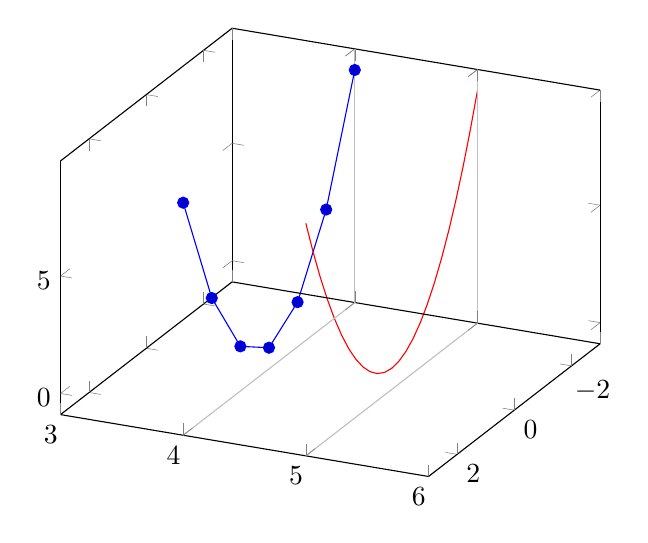
\begin{tikzpicture}
\begin{axis}[
    xmin=3,xmax=6,
    extra x ticks={4,5},
    extra x tick style={xticklabel=\empty,grid=major}
]
    \addplot3 table [x expr=4,y=a,z=b] {
        a  b
        -3 9
        -2 4
        -1 1
        0  0
        1  1
        2  4
        3  9
    };
    \addplot3 [red,domain=-3:3,samples y=1] (5,x,x^2);
\end{axis}
\end{tikzpicture}
\end{codeexample}
%
\noindent 这里，我们在一个坐标轴中有两个图：一个来自数据表的数据图
（仅有两个坐标）和一个参数图。两者表示相同的两个函数。对于数据图，
|x expr=4| 分配 $x$ 坐标，|y=a,z=b| 定义输入列如何映射到坐标。
同样，该图隐式使用 |mesh/rows=1|，因为没有扫描线结束标记。第二个图
使用简写符号 |(5,x,x^2)| 做同样的事情。由于 |samples y=1|，它仅
采样一维数据。最后，|extra x ticks| 为 $x$ 轴配置两个额外的刻度；
这用于为这些特定刻度显示网格线。|xticklabel=\empty| 参数避免在位置
$x\in\{4,5\}$ 处重叠的 $x$ 刻度标签。

三维线图通常会使用线来连接点（即 \Tikz 的初始 |sharp plot| handler）。
\Tikz 的 |smooth| 方法也可能是一个选项。注意，三维坐标轴不支持分段
常值图、梳状图或柱状图 handler。


\subsubsection{3D 中的填充线图}
\label{sec:pgfplots:filled:line}

闭合线图也适用于三维坐标轴。其工作方式与 \ref{sec:pgfplots:closingplots}
节中为二维坐标轴概述的相同：通过使用 |\closedcycle|。

\begin{codeexample}[]
\begin{tikzpicture}
\pgfplotstableread{
plot1     plot2     plot3     plot4
0.0045    0.0029    0.0089    0.0001
0.0024    0.0023    0.0050    0.0016
0.0007    0.0012    0.0010    0.0001
0.0000    0.0004   -0.0000   -0.0015
0.0001    0.0001    0.0007   -0.0021
0.0003    0.0000    0.0015   -0.0020
0.0003    0.0001    0.0017   -0.0018
0.0003    0.0001    0.0016   -0.0015
0.0003    0.0001    0.0016   -0.0013
0.0003    0.0002    0.0015   -0.0012
}\tabledata
\begin{axis}[
    zmin=-0.001,
    area plot/.style={
        fill opacity=0.75,
        draw=orange!80!black,thick,
        fill=orange,
        mark=none,
    },
    ytick={1,...,4},
    yticklabel=plot\pgfmathprintnumber{\tick},
]
    \pgfplotsinvokeforeach{4,3,...,1}{
        \addplot3 [area plot] table [
            x expr=\coordindex, y expr=#1, z=plot#1,
        ] {\tabledata} \closedcycle;
    }
\end{axis}
\end{tikzpicture}
\end{codeexample}

这里的区别在于 \PGFPlots{} 将连接 $z=0$ 平面上的第一个和最后一个
坐标；如果 $z=0$ 在坐标轴限制之外，则连接 $z_{\min}$
平面上的坐标。


\subsection{散点图}

三维散点图与二维
散点图具有相同的接口，因此 \ref{sec:pgfplots:scatter:2d} 节的所有示例也可用于三维
情况。关键功能是使用 |only marks| 和/或 |scatter| 作为绘图样式。

我们提供一些专门针对三维情况的示例。

我们的第一个示例使用 |only marks| 在每个输入位置放置当前绘图 |mark|：
%
\pgfplotsexpensiveexample
\begin{codeexample}[]
\begin{tikzpicture}
\begin{axis}[
    xlabel=$x$,
    ylabel=$y$,
    zlabel={$f(x,y) = x\cdot y$},
    title=A Scatter Plot Example,
]
    % `pgfplotsexample4_grid.dat' contains a
    % large sequence of input points of the form
    % x_0   x_1     f(x)
    % 0     0       0
    % 0     0.03125 0
    % 0     0.0625  0
    % 0     0.09375 0
    % 0     0.125   0
    % 0     0.15625 0
    \addplot3+ [only marks]
        table {plotdata/pgfplotsexample4_grid.dat};
    \end{axis}
\end{tikzpicture}
\end{codeexample}

如果我们添加键 |scatter|，绘图标记还将使用当前 |colormap| 的颜色：
%
\pgfplotsexpensiveexample
\begin{codeexample}[]
\begin{tikzpicture}
\begin{axis}[
    xlabel=$x$,
    ylabel=$y$,
    zlabel={$f(x,y) = x\cdot y$},
    title=A Scatter Plot Example,
]
    \addplot3+ [
        only marks,
        scatter,
    ] table {plotdata/pgfplotsexample4_grid.dat};
\end{axis}
\end{tikzpicture}
\end{codeexample}

一个更复杂的示例是将近似函数绘制为 |surf| 图（需要矩阵数据），并将
底层网格（即 |scatter| 的数据）放置到同一坐标轴中。我们选择将
$(x,y)$ 网格点放置在 $z=1.4$ 处。此外，我们希望网格点根据输入表中
|f(x)| 列的值着色：

\pgfplotsexpensiveexample
\begin{codeexample}[]
\begin{tikzpicture}
    \begin{axis}[
        3d box,
        zmax=1.4,
        colormap/viridis,
        colorbar,
        xlabel=$x$,
        ylabel=$y$,
        zlabel={$f(x,y) = x\cdot y$},
        title={Using Coordinate Filters to fix $z=1.4$},
    ]
        % `pgfplotsexample4.dat' contains similar data as in
        % `pgfplotsexample4_grid.dat', but it uses a uniform
        % matrix structure (same number of points in every scanline).
        % See examples above for extracts.
        \addplot3 [surf,mesh/ordering=y varies]
            table {plotdata/pgfplotsexample4.dat};
        \addplot3 [scatter,scatter src=\thisrow{f(x)},only marks, z filter/.code={\def\pgfmathresult{1.4}}]
            table {plotdata/pgfplotsexample4_grid.dat};
    \end{axis}
\end{tikzpicture}
\end{codeexample}
%
\noindent 我们使用 |z filter| 将 $z$ 坐标固定为 $1.4$。我们也可以使用
|table/z expr=1.4| 功能
%
\begin{codeexample}[code only]
    \addplot3 [scatter,scatter src=\thisrow{f(x)},only marks]
        table [z expr=1.4] {plotdata/pgfplotsexample4_grid.dat};
\end{codeexample}
%
\noindent 来获得完全相同的效果。选择你最喜欢的方式。|z filter| 适用于
每个坐标输入例程，而 |z expr| 功能仅适用于 |\addplot table|。

以下示例使用 |mark=cube*| 和 |z buffer=sort| 在每个输入坐标处放置
立方体。每个立方体的颜色由 |point meta={x+y+3}| 确定。其余键仅用于
美观打印。
%
\pgfplotsexpensiveexample
\begin{codeexample}[]
\begin{tikzpicture}
    \begin{axis}[
        view={120}{40},
        width=220pt,
        height=220pt,
        grid=major,
        z buffer=sort,
        xmin=-1,xmax=9,
        ymin=-1,ymax=9,
        zmin=-1,zmax=9,
        enlargelimits=upper,
        xtick={-1,1,...,19},
        ytick={-1,1,...,19},
        ztick={-1,1,...,19},
        xlabel={$l_1$},
        ylabel={$l_2$},
        zlabel={$l_3$},
        point meta={x+y+z+3},
        colormap={summap}{
            color=(black)  color=(blue)
            color=(black)  color=(white)
            color=(orange) color=(violet)
            color=(red)
        },
        scatter/use mapped color={
            draw=mapped color,fill=mapped color!70},
        ]
        % `pgfplots_scatter4.dat' contains a large sequence of
        % the form
        % l_0   l_1     l_2
        % 1     6       -1
        % -1    -1      -1
        % 0     -1      -1
        % -1    0       -1
        % -1    -1      0
        % 1     -1      -1
        % 0     0       -1
        % 0     -1      0
        \addplot3 [only marks,scatter,mark=cube*,mark size=7]
            table {plotdata/pgfplots_scatterdata4.dat};
    \end{axis}
\end{tikzpicture}
\end{codeexample}


\subsection{网格图}
\label{sec:2d:mesh}

\begin{plottype}[/pgfplots]{mesh}
    网格图对每个网格段使用不同的颜色。颜色使用"颜色坐标"确定，在本文
    档中也称为"元数据"。这与用于曲面图和散点图的数据相同，参见
    \ref{pgfplots:pointmeta} 节。在初始配置中，"颜色坐标"是 $z$ 轴
    （对于二维图是 $y$ 轴）。该颜色坐标被线性映射到当前颜色图中，以
    确定每个网格段的颜色。因此，如果出现的最小颜色数据比如是 $-1$，
    最大是 $42$，则颜色数据为 $-1$ 的点将获得颜色图下端的颜色，颜色
    数据为 $42$ 的点获得颜色图上端的颜色。

\pgfplotsexpensiveexample
\begin{codeexample}[]
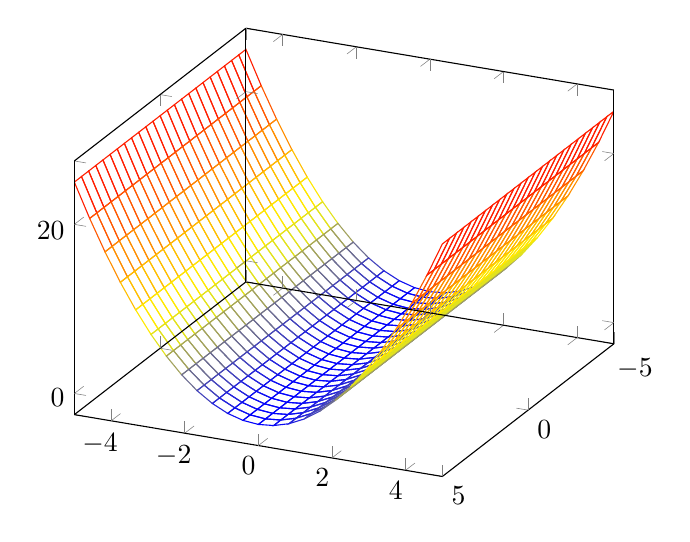
\begin{tikzpicture}
\begin{axis}
    \addplot3 [mesh] {x^2};
\end{axis}
\end{tikzpicture}
\end{codeexample}

    网格图可以与标记或 |scatter| 键组合，后者也以不同颜色绘制标记。

\pgfplotsexpensiveexample
\begin{codeexample}[]
% requires \usepgfplotslibrary{colorbrewer}
\begin{tikzpicture}
\begin{axis}[
    colormap/PuOr,
]
    \addplot3+ [
        mesh,
        scatter,
        samples=10,
        domain=0:1,
    ] {x*(1-x)*y*(1-y)};
\end{axis}
\end{tikzpicture}
\end{codeexample}

\pgfplotsexpensiveexample
\begin{codeexample}[]
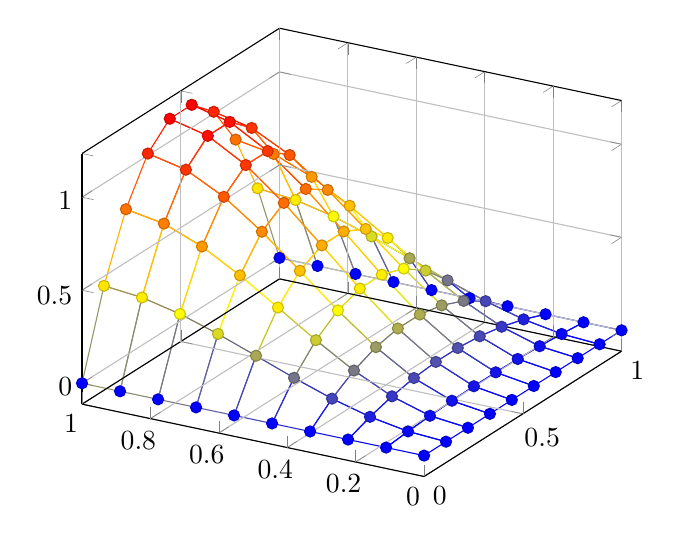
\begin{tikzpicture}
\begin{axis}[
    grid=major,
    view={210}{30},
]
    \addplot3+ [
        mesh,
        scatter,
        samples=10,
        domain=0:1,
    ] {5*x*sin(2*deg(x)) * y*(1-y)};
\end{axis}
\end{tikzpicture}
\end{codeexample}

    有时，可能希望隐藏背景网格段。这可以使用 |surf| plot handler
    （见下文）和特定填充颜色来实现：
    %
\pgfplotsexpensiveexample
\begin{codeexample}[]
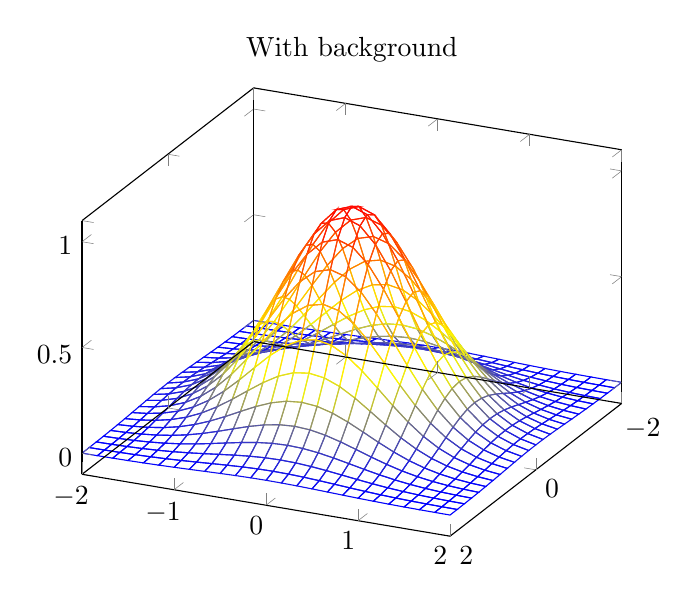
\begin{tikzpicture}
    \begin{axis}[title=With background]
        \addplot3 [mesh,domain=-2:2] {exp(-x^2-y^2)};
    \end{axis}
\end{tikzpicture}
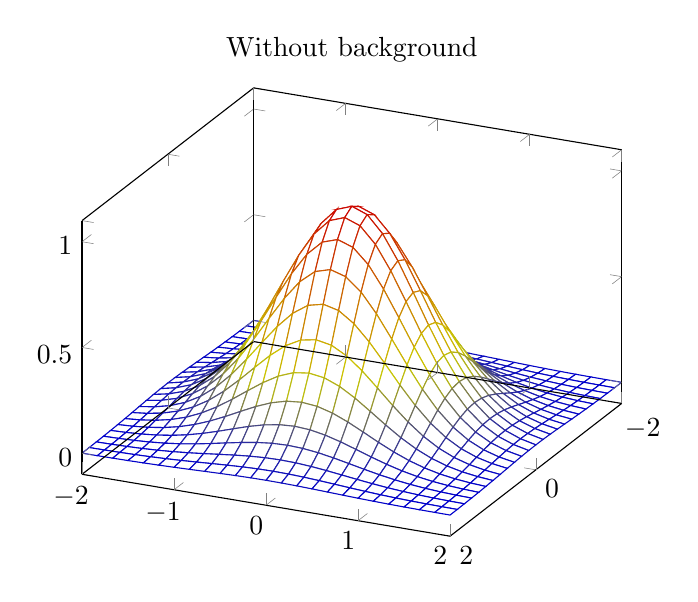
\begin{tikzpicture}
    \begin{axis}[title=Without background]
        \addplot3 [surf,fill=white,domain=-2:2] {exp(-x^2-y^2)};
    \end{axis}
\end{tikzpicture}
\end{codeexample}
    %
    填充颜色需要显式提供。


    \paragraph{细节：}

    \begin{itemize}
        \item 网格图使用与 |shader=flat| 相同的实现来为每个单段获得
            一种颜色。因此，如果 |shader=flat mean|，一个段的颜色使用
            相邻顶点颜色数据的\emph{平均值}确定。如果
            |shader=flat corner|，一个段的颜色是\emph{第一个}相邻顶点
            的颜色。\footnote{从 \PGFPlots{} 1.13 及相关兼容级别开始，
            即使在存在 $z$ 缓冲的情况下也是如此。}
        \item 一旦激活 |mesh|，就会安装 |color=mapped color|。这是
            \emph{必要的}，除非需要不同的颜色——但 |mapped color| 是
            唯一反映颜色数据的颜色。

            可以像任何其他图一样使用 |color=|\meta{color name} 来使用
            不同的颜色。
        \item 很容易向网格图添加 |mark=|\meta{marker name}，也可以使用
            |scatter|。散点图将使用与网格相同的颜色数据。
    \end{itemize}

\pgfplotsexpensiveexample
\begin{codeexample}[]
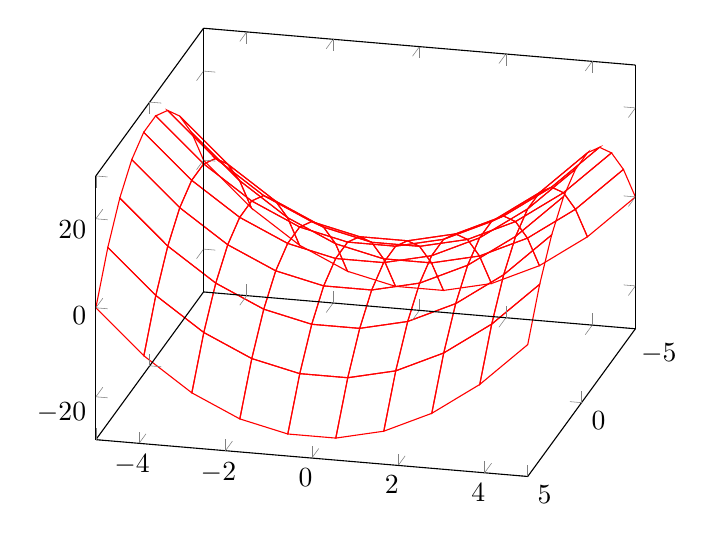
\begin{tikzpicture}
\begin{axis}[view/az=14]
    \addplot3 [
        mesh,
        draw=red,
        samples=10,
    ] {x^2-y^2};
\end{axis}
\end{tikzpicture}
\end{codeexample}

    网格图使用 |mesh legend| 样式来排版图例图像。
\end{plottype}

\begin{pgfplotskey}{mesh/check=\mchoice{false,warning,error} (initially error)}
    允许配置当 |mesh/rows| $\times$ |mesh/cols| 不等于坐标总数时是否
    生成错误。

    如果你确切地知道自己在做什么，禁用检查可能很有用。如果不确定，
    最好保留初始设置。
\end{pgfplotskey}

\begin{pgfplotskey}{z buffer=\mchoice{%
        default,
        none,
        auto,
        sort,
        reverse x seq,
        reverse y seq,
        reverse xy seq%
    } (initially default)%
}
    此键允许在不同的 $z$ 缓冲策略之间进行选择。$z$ 缓冲决定图像的哪些
    部分应绘制在其他部分前面。由于图形包 \PGF{} 和最终文档格式
    |.pdf| 本质上都是二维的，这项工作必须在 \TeX{} 中完成。目前，可以
    使用几种（快速）启发式方法，它们对于简单的网格和曲面图效果相当好。
    此外，还有一种（耗时的）排序方法，当快速启发式方法失败时也能工作。

    \PGFPlots{} 的 $z$ 缓冲算法仅适用于单个 |\addplot| 命令。不同的
    |\addplot| 命令将按出现顺序彼此叠绘。

    选项 \declaretext{default} 检查我们当前是否处理网格或曲面图，并在
    这种情况下使用 |auto|。如果不是，它设置 |z buffer=none|。

    选项 \declaretext{none} 禁用 $z$ 缓冲。对于不需要 $z$ 缓冲的二维
    坐标轴也是如此。

    选项 \declaretext{auto} 是任何网格或曲面图的初始值：它使用非常
    快速的启发式方法来决定如何为网格和曲面图执行 $z$ 缓冲。其思想是
    反转所有 $x$ 坐标的序列，或所有 $y$ 坐标的序列，或两者。对于
    规则网格，这足以提供 $z$ 缓冲。换句话说，选项 |auto| 将使用三种
    反转策略 |reverse |*| seq| 之一（或根本不使用）。应用于 |patch|
    图的选项 |auto| 使用 |z buffer=sort|，因为 |patch| 图没有矩阵结构。

    选项 \declaretext{sort} 可用于散点图、线图、网格图、曲面图和补丁图。
    它根据每个点（或网格段）的深度排序。在 \TeX{} 中排序使用慢速算法，
    可能需要大量内存（尽管它具有预期的运行时间渐近性
    $\mathcal O(N \log N)$）。网格段的深度只是\emph{一个}数字，目前
    确定为顶点深度的\emph{平均值}。由于 |z buffer=sort| 实际上只是
    一种更智能地将网格段彼此叠绘的方式，它仍可能失败。如果网格段很大
    且在段的不同部分重叠，可能会发生失败（参见维基百科"Painter's
    algorithm"）。如果遇到此类问题，考虑减小网格宽度（网格元素大小），
    使它们可以独立排序（例如使用 |patch refines=2| 自动进行，参见
    |patchplots| 库）。

    其余选项仅适用于网格/曲面图（即矩阵数据），并且除了其名称所指示的
    之外不做更多事情：它们反转输入矩阵的坐标序列（使用拟线性运行时间）。
    它们应仅与 |z buffer=auto| 结合使用。
\end{pgfplotskey}


\subsection{曲面图}
\label{sec:pgfplots:surfplots}

\begin{plottype}[/pgfplots]{surf}
    曲面图使用不同的填充颜色为每个补丁段可视化一个二维单补丁。每个
    补丁段是一个（伪）矩形，这意味着输入数据以数据矩阵的形式给出，
    如关于三维坐标的介绍性 \ref{sec:pgfplots:sec:threedim} 节所讨论。

\pgfplotsexpensiveexample
\begin{codeexample}[]
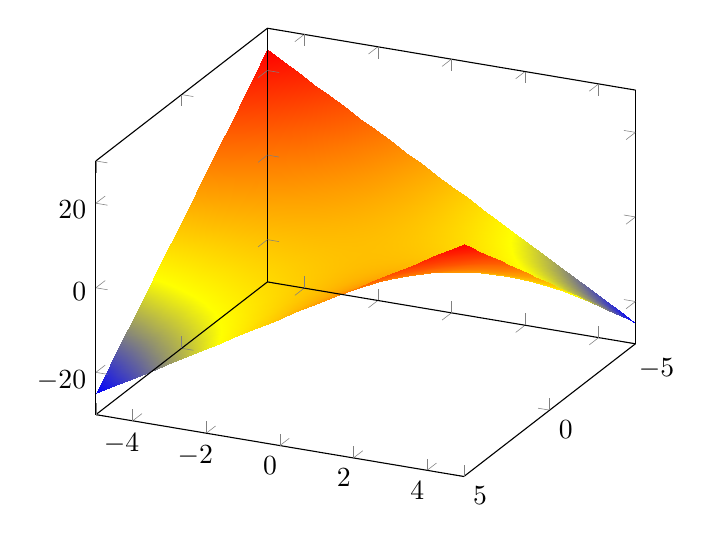
\begin{tikzpicture}
\begin{axis}
    \addplot3 [
        surf,
        shader=interp,
    ] {x*y};
\end{axis}
\end{tikzpicture}
\end{codeexample}

    生成曲面图最简单的方式是使用 plot expression 功能，但是——如
    \ref{sec:pgfplots:sec:threedim} 节所讨论的——其他输入方法如
    \verbpdfref{\addplot3 table} 或
    \verbpdfref{\addplot3 coordinates} 也是可能的。

    外观可以使用 |colormap|、|point meta| 的值以及
    |shader| 键来配置，见下文。对于面，安装了特殊的 |color=mapped color|
    （如 |mesh| 图一样）。带刻面图的描边颜色可以用 |faceted color|
    设置（详见下文）。

\pgfplotsexpensiveexample
\begin{codeexample}[]
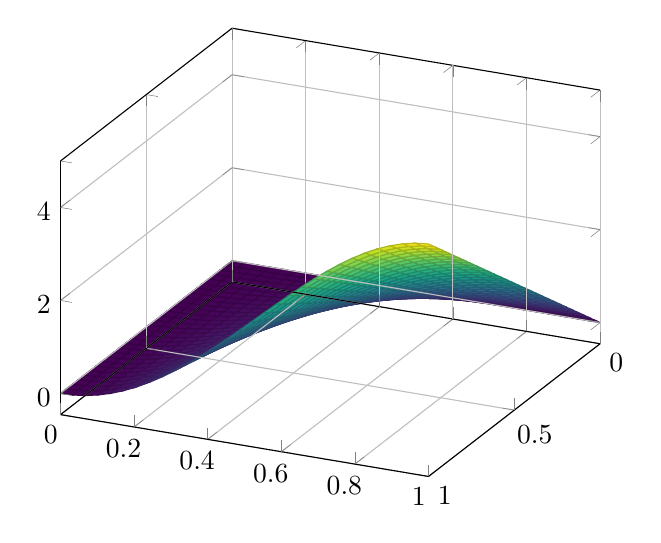
\begin{tikzpicture}
\begin{axis}[
    grid=major,
    colormap/viridis,
]
    \addplot3 [
        surf,
        samples=30,
        domain=0:1,
    ] {5*x*sin(2*deg(x)) * y};
\end{axis}
\end{tikzpicture}
\end{codeexample}

\pgfplotsexpensiveexample
\begin{codeexample}[]
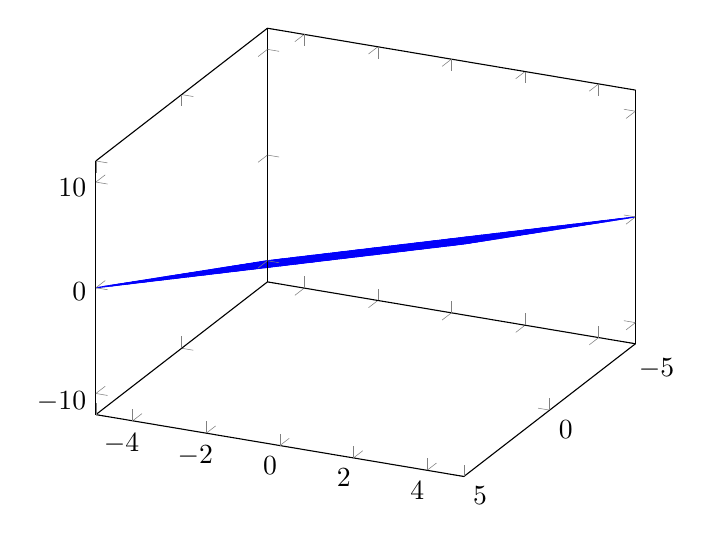
\begin{tikzpicture}
\begin{axis}
    \addplot3 [
        surf,
        faceted color=blue,
    ] {x+y};
\end{axis}
\end{tikzpicture}
\end{codeexample}

\pgfplotsexpensiveexample
\begin{codeexample}[]
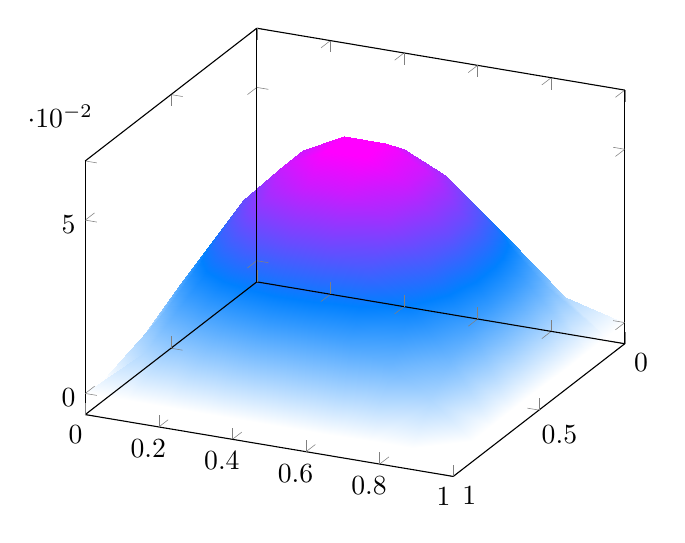
\begin{tikzpicture}
    \begin{axis}[colormap/cool]
        \addplot3 [surf,samples=10,domain=0:1,shader=interp]
            {x*(1-x)*y*(1-y)};
    \end{axis}
\end{tikzpicture}
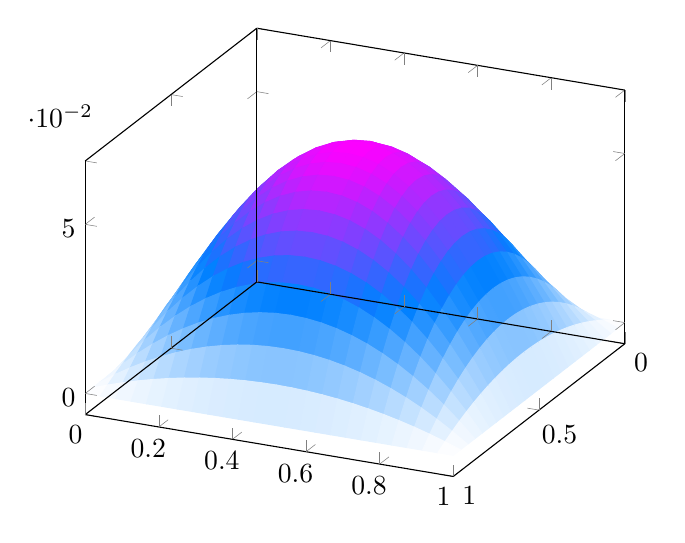
\begin{tikzpicture}
    \begin{axis}[colormap/cool]
        \addplot3 [surf,samples=25,domain=0:1,shader=flat]
            {x*(1-x)*y*(1-y)};
    \end{axis}
\end{tikzpicture}
\end{codeexample}

\pgfplotsexpensiveexample
\begin{codeexample}[]
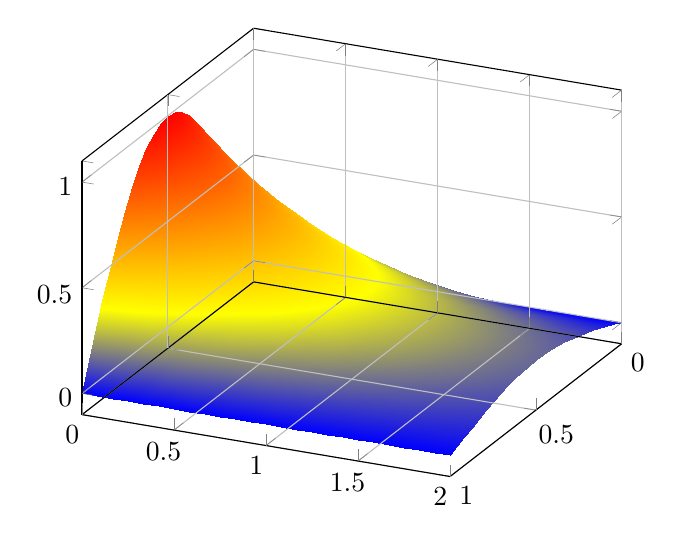
\begin{tikzpicture}
\begin{axis}[grid=major]
    \addplot3 [
        surf,
        shader=interp,
        samples=25,
        domain=0:2,
        y domain=0:1,
    ] {exp(-x) * sin(pi*deg(y))};
\end{axis}
\end{tikzpicture}
\end{codeexample}

\pgfplotsexpensiveexample
\begin{codeexample}[]
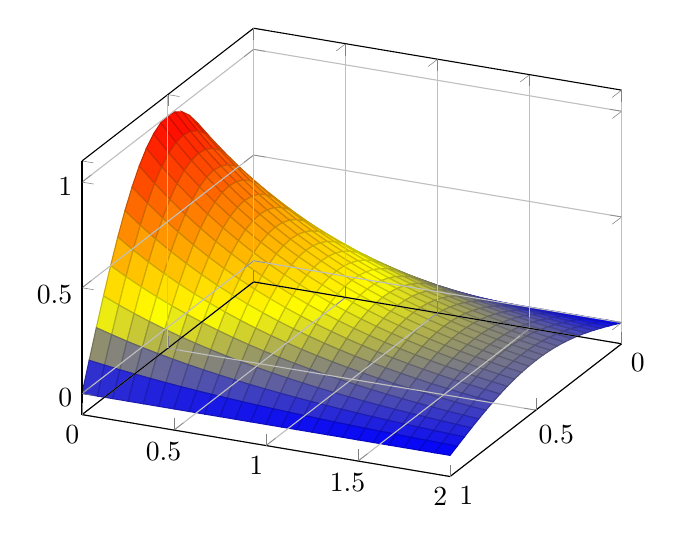
\begin{tikzpicture}
\begin{axis}[grid=major]
    \addplot3 [
        surf,
        shader=faceted,
        samples=25,
        domain=0:2,
        y domain=0:1,
    ] {exp(-x) * sin(pi*deg(y))};
\end{axis}
\end{tikzpicture}
\end{codeexample}

    关于着色算法的详情在下文 |shader| 的文档中提供。

    曲面图使用 |mesh legend| 样式来创建图例图像。
\end{plottype}

\begin{pgfplotskey}{shader=\mchoice{%
        flat,
        interp,
        faceted,
        flat corner,
        flat mean,
        faceted interp%
    } (initially faceted)%
}
    配置用于曲面图的着色器。着色器决定每个单顶点处可用的颜色数据如何
    用于填充曲面补丁。

    最简单的选择是为每个段使用一种填充颜色，即选项
    \declareandlabel{flat}。

\pgfplotsexpensiveexample
\begin{codeexample}[]
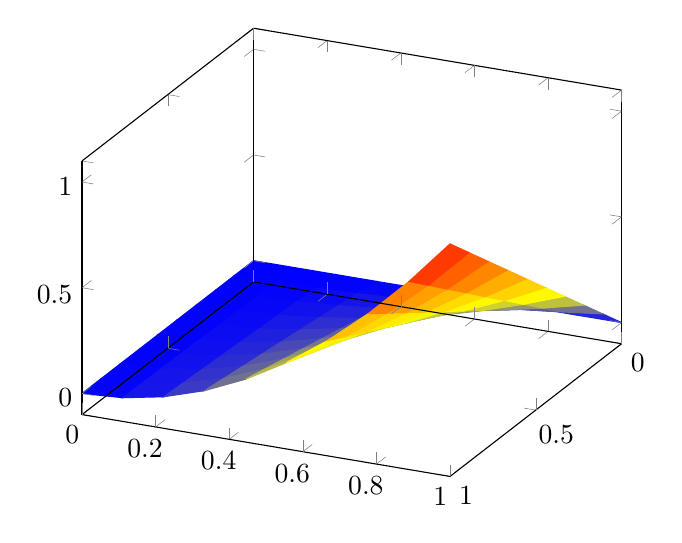
\begin{tikzpicture}
\begin{axis}
    \addplot3 [
        surf,
        shader=flat,
        samples=10,
        domain=0:1,
    ] {x^2*y};
\end{axis}
\end{tikzpicture}
\end{codeexample}

    \noindent （目前）有两种可能性来确定每个段的单一颜色：
    %
    \begin{description}
        \item[\declaretext{flat corner}] 使用一个顶点的颜色数据为该段
            着色。\emph{第一个}顶点的颜色决定整个段的颜色。注意，
            \PGFPlots{} 确保结果始终相同，即使顶点由于 |z buffer| 或
            |mesh/ordering| 而被重新排序。

            注意，\PGFPlots{} 1.12 及更早版本选择其中一个而不考虑
            重新排序。为了使排序独立于其他功能，你必须写入
            |compat=1.13| 或更新版本。
        \item[\declaretext{flat mean}] 使用所有四个颜色数据值的平均值
            作为段颜色。这是初始值，因为它为对称函数提供对称颜色。
    \end{description}
    %
    选项 |flat| 实际上与 |flat mean| 相同。请注意，|shader=flat mean|
    和 |shader=flat corner| 也影响网格图——这些选项决定网格段颜色。

    另一个选择是 |shader=|\declareandlabel{interp}，它使用 Goraud 着色
    （两个三角形的平滑线性插值近似矩形）来填充段。

\pgfplotsexpensiveexample
\begin{codeexample}[]
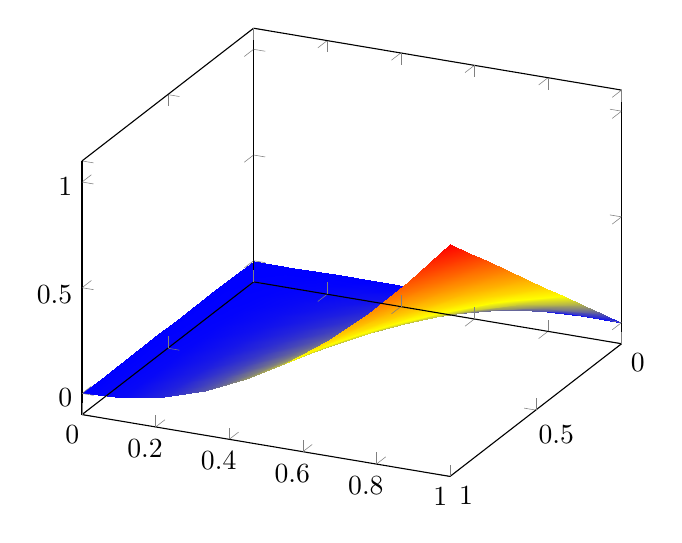
\begin{tikzpicture}
\begin{axis}
    \addplot3 [
        surf,
        shader=interp,
        samples=10,
        domain=0:1,
    ] {x^2*y};
\end{axis}
\end{tikzpicture}
\end{codeexample}

    |shader=interp| 使用底层着色实现，目前适用于以下驱动：
    %
    \begin{itemize}
        \item postscript 驱动 |\def\pgfsysdriver{pgfsys-dvips.def}|，
        \item |pdflatex| 驱动 |\def\pgfsysdriver{pgfsys-pdftex.def}|，
        \item |lualatex| 驱动 |\def\pgfsysdriver{pgfsys-pdftex.def}| 和
            \\ |\def\pgfsysdriver{pgfsys-luatex.def}|，
        \item |dvipdfmx| 驱动 |\def\pgfsysdriver{pgfsys-dvipdfmx.def}|。
    \end{itemize}
    %
    对于其他驱动，选项 |shader=interp| 将产生警告，并且等同于
    |shader=flat mean|。另见下文的详细说明。

    注意，|shader=interp,patch type=bilinear| 允许真正的双线性插值，
    参见 |patchplots| 库。

    选项 |shader=|\declareandlabel{faceted} 为每个网格段使用常量填充
    颜色（如 |flat|），并使用键 |/pgfplots/faceted color| 的值来绘制
    连接的网格元素：
    %
\pgfplotsexpensiveexample
\begin{codeexample}[]
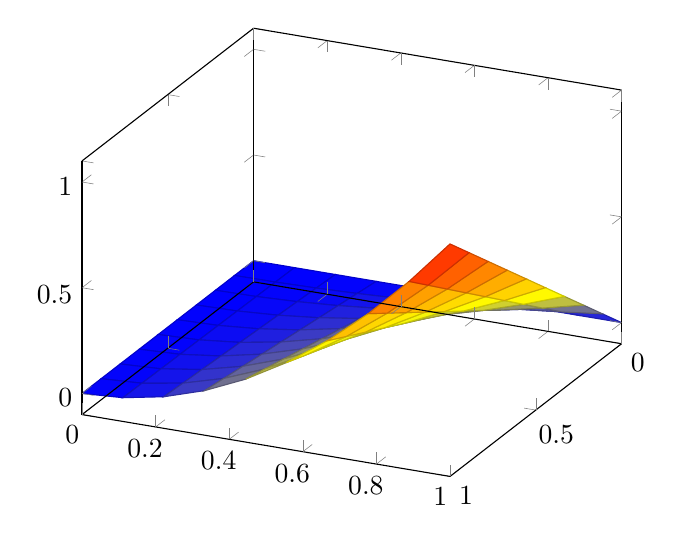
\begin{tikzpicture}
\begin{axis}
    \addplot3 [
        surf,
        shader=faceted,
        samples=10,
        domain=0:1,
    ] {x^2*y};
\end{axis}
\end{tikzpicture}
\end{codeexample}

    最后一个选项是 |shader=|\declareandlabel{faceted interp}。顾名思义，
    它是 |interp| 和 |faceted| 的混合，即每个元素使用线性三角形插值
    着色（关于双线性插值，另见 |patchplots| 库），方式与 |interp|
    相同，但此外，边缘以 |faceted color| 着色：
    %
\pgfplotsexpensiveexample
\begin{codeexample}[]
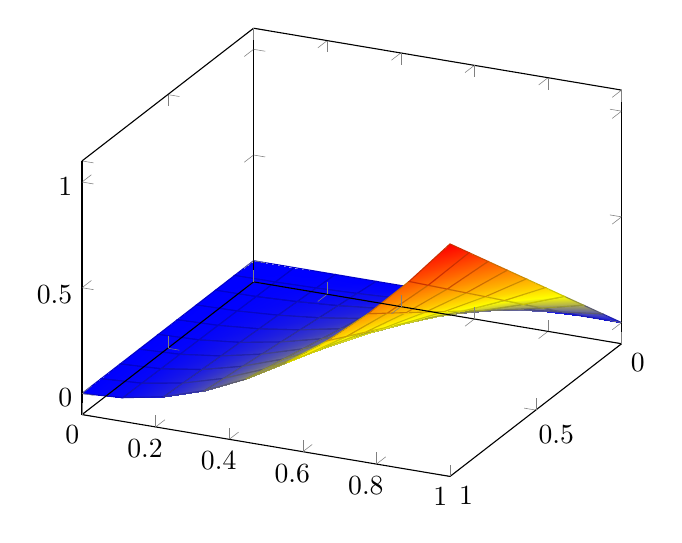
\begin{tikzpicture}
\begin{axis}
    \addplot3 [
        surf,
        shader=faceted interp,
        samples=10,
        domain=0:1,
    ] {x^2*y};
\end{axis}
\end{tikzpicture}
\end{codeexample}
    %
    \noindent 原则上，这个想法本身没有问题，而且看起来相当不错——但它
    会显著增大生成的 PDF 文档，并且可能需要很长时间来渲染。其工作方式
    如下：对于每个网格元素（|patch| 图的三角形或晶格图的矩形），
    它创建一个底层着色。然后它用该着色填充单个网格元素，并用
    |faceted color| 描边边缘。声明如此多的底层着色在 PDF 对象方面
    相当低效（输出文件大），并且可能渲染缓慢。\footnote{我的经验如下：
    Acrobat reader 可以高效渲染巨大的 \texttt{interp} 着色。但它对
    \texttt{faceted interp} 着色非常慢。Linux 查看器如 xpdf 对
    \texttt{interp} 相当高效（至少在我对 libpoppler 的错误修复下），
    并且对 \texttt{faceted interp} 着色也很快。} 对于正交图
    （如 |view={0}{90}|），如果使用两个单独的 |\addplot| 命令：一个
    用 |surf|，一个用 |mesh|，则可以以较少的代价获得
    |faceted interp| 的效果。请谨慎处理此选择。


    \paragraph{细节：}

    \begin{itemize}
        \item 所有着色器都支持 |z buffer=sort|（从 1.4 版本开始）。
        \item 选项 |shader=faceted| 与 |shader=flat| 相同——除了它使用
            特殊的绘制颜色。

            因此，|shader=faceted| 的效果与

            |shader=flat,draw=\pgfkeysvalueof{/pgfplots/faceted color}|
            相同。
        \item |flat| 着色器使用当前的 |draw| 和 |fill| 颜色。它们通过
            |color=mapped color| 设置，可以用 |draw=|\meta{draw color}
            和 |fill=|\meta{fill color} 覆盖。|mapped color| 始终包含
            颜色图的颜色。
        \item 你可以轻松地向网格和/或曲面图添加
            |mark=|\meta{plot mark}，甚至使用 |scatter| 的彩色绘图标记。
            散点图功能将使用与曲面相同的颜色数据。

            但是：标记和曲面不共享相同的深度信息。它们彼此叠绘。
        \item 关于 |shader=interp| 的备注：
            %
            \begin{itemize}
                \item 它在任何情况下都使用当前颜色图，忽略
                    |draw| 和 |fill|。
                \item 对于具有大量点的曲面图，|shader=interp| 产生
                    更小的 |pdf| 文档，在 \TeX{} 中需要更少的编译时间，
                    并且在 Acrobat Reader 中显示所需时间比
                    |shader=flat| 更少。
                \item postscript 驱动\emph{将}坐标\emph{截断}到
                    24~bit——这可能导致精度损失（截断不是很智能）。
                    详情参见 |surf shading/precision| 键。为了提高
                    兼容性，这种 24 位截断算法也默认对 PDF 文档启用。
                \item 选项 |shader=interp| 与 Acrobat Reader 或最新
                    版本的免费查看器配合良好。\footnote{本包的作者已
                    向 xpdf/libpoppler 提交了错误修复，这些修复应该
                    是许多查看器当前稳定版本的一部分。} 但是，一些
                    免费查看器错误地显示颜色（如 evince）。我希望这条
                    消息很快会过时\ldots{} 如果没有，请向 Linux
                    社区提供错误报告，以传达需要改进对 Type 4
                    （|patch|）和 Type 5 PDF（|surf|）以及 Type 7
                    （|patch| 和 |patchplots| 库的元素）着色的支持。
                \item |interp| 着色器产生与
                    |faceted interp,faceted color=none| 相同的结果，
                    尽管 |faceted interp| 需要更多资源。
            \end{itemize}
    \end{itemize}

\pgfplotsexpensiveexample
\begin{codeexample}[]
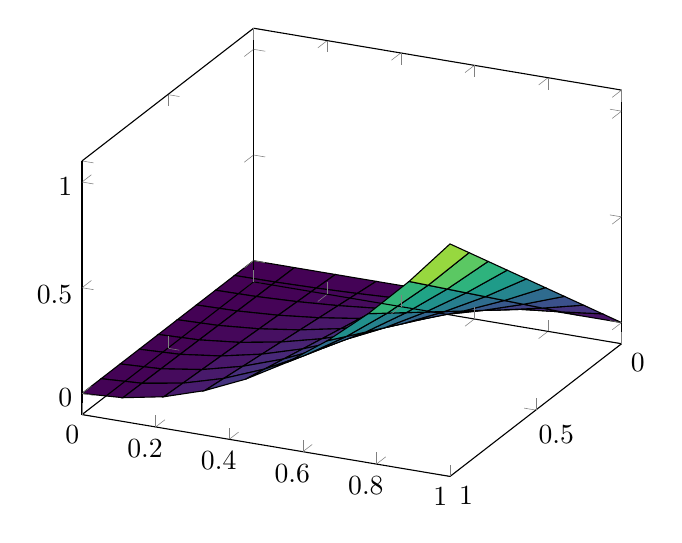
\begin{tikzpicture}
\begin{axis}[colormap/viridis]
    \addplot3 [
        surf,
        shader=flat,
        draw=black,
        samples=10,
        domain=0:1,
    ] {x^2*y};
\end{axis}
\end{tikzpicture}
\end{codeexample}

\pgfplotsexpensiveexample
\begin{codeexample}[]
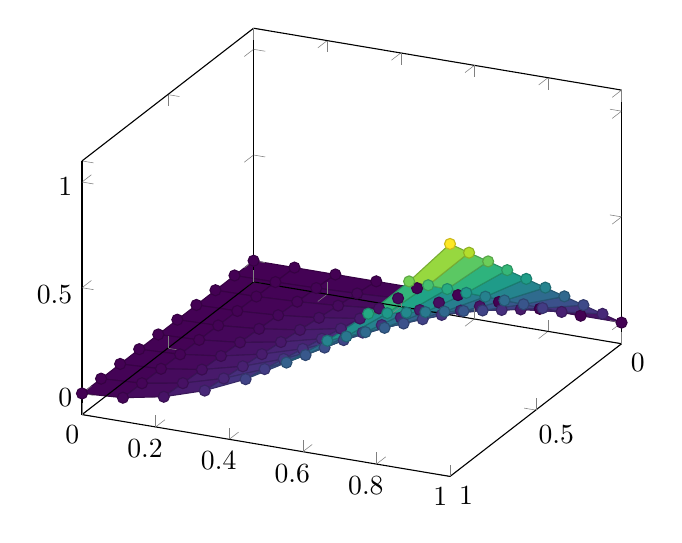
\begin{tikzpicture}
\begin{axis}[colormap/viridis]
    \addplot3 [
        surf,
        shader=faceted,
        scatter,mark=*,
        samples=10,
        domain=0:1,
    ] {x^2*y};
\end{axis}
\end{tikzpicture}
\end{codeexample}

    注意，|shader| 始终与 |colormap access| 交互。特别是，
    |colormap access=piecewise constant| 与 |shader=interp| 结合会
    产生填充等高线图，详情参见 \ref{sec:pgfplots:filled:contour} 节。
\end{pgfplotskey}

\begin{pgfplotskey}{faceted color=\marg{color name} (initially mapped color!80!black)}
    定义用于带刻面曲面图的网格的颜色。

    设置 |faceted color=none| 以禁用边缘颜色。
\end{pgfplotskey}

{
\tikzset{
    external/figure name/.add={}{interior_colormap_},
    /pdflinks/search key prefixes in/.add={}{,/pgfplots/mesh/},
}%
\begin{pgfplotskeylist}{%
    mesh/interior colormap=\marg{map name}\marg{colormap specification},%
    mesh/interior colormap name=\marg{map name}%
}
    允许为曲面的"另一侧"使用不同的 |colormap|。

    每个网格有两面：一面"指向"视图原点，另一面背向它。此键允许为
    背向视图原点的一面定义第二个 |colormap|。其动机是区分曲面的外侧
    和内部部分：
    %
\pgfplotsexpensiveexample
\begin{codeexample}[]
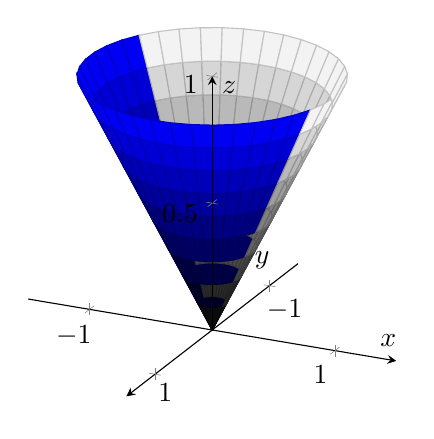
\begin{tikzpicture}
\begin{axis}[
    axis lines=center,
    axis on top,
    xlabel={$x$}, ylabel={$y$}, zlabel={$z$},
    domain=0:1,
    y domain=0:2*pi,
    xmin=-1.5, xmax=1.5,
    ymin=-1.5, ymax=1.5, zmin=0.0,
    mesh/interior colormap=
        {blueblack}{color=(black) color=(blue)},
    colormap/blackwhite,
    samples=10,
    samples y=40,
    z buffer=sort,
]
    \addplot3 [surf]
        ({x*cos(deg(y))},{x*sin(deg(y))},{x});
\end{axis}
\end{tikzpicture}
\end{codeexample}

    \noindent The |interior colormap| is often the one for the ``inner side''.
    但是，曲面的方向取决于其法线向量：\PGFPlots{} 使用右手定则计算
    它们。应用于三角形的右手定则意味着取第一个遇到的点，拇指指向
    第二个点的方向，食指指向第三个点的方向。那么，该三角形的法线
    就是中指（即所涉及的有向边的叉积）。对于矩形补丁，它们被
    分解为两个三角形，并且法线按上述方式确定。
    （即所涉及的有向边的叉积）。对于矩形补丁，\PGFPlots{} 使用其
    一个三角形的法线。\footnote{这在未来版本中可能会改变。}
    因此，|mesh/interior colormap| 仅在所涉及的补丁段方向一致时
    才有效。

    法线向量指向与视图方向相同方向的补丁使用标准 |colormap name|。
    法线向量指向相反方向（即指向视口方向）的补丁使用
    |mesh/interior colormap|。

\pgfplotsexpensiveexample
\begin{codeexample}[]
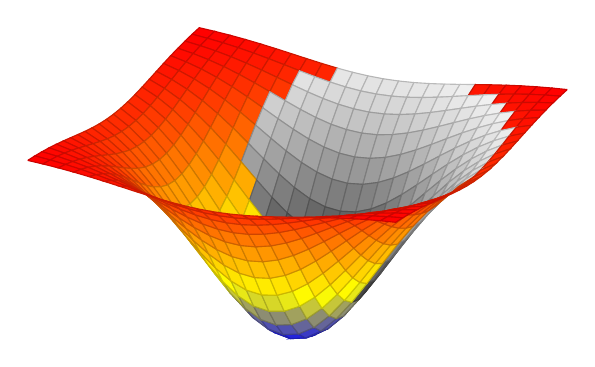
\begin{tikzpicture}
\begin{axis}[
    hide axis,
    xlabel=$x$,ylabel=$y$,
    mesh/interior colormap name=hot,
    colormap/blackwhite,
]
    \addplot3 [domain=-1.5:1.5,surf]
        {-exp(-x^2-y^2)};
\end{axis}
\end{tikzpicture}
\end{codeexample}

    |mesh/interior colormap| 的实现对大多数示例效果良好；特别是当样本
    数量足够大以分辨内、外颜色图之间的边界时。但是，它仍可能产生虚假
    伪影：
    %
\pgfplotsexpensiveexample
\begin{codeexample}[]
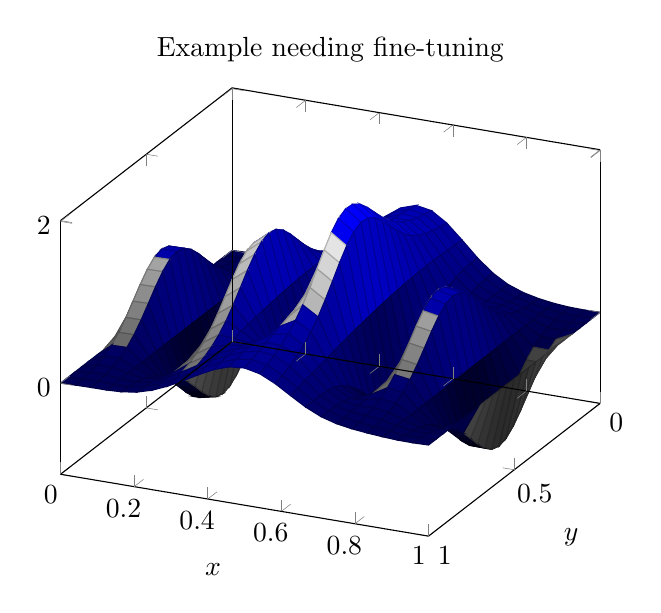
\begin{tikzpicture}
\begin{axis}[
    title=Example needing fine-tuning,
    xlabel=$x$,
    ylabel=$y$,
]
    \addplot3 [surf,
        mesh/interior colormap={blueblack}{
            color=(black) color=(blue)
        },
        colormap/blackwhite,
        domain=0:1,
    ] {
        sin(deg(8*pi*x))* exp(-20*(y-0.5)^2)
            + exp(-(x-0.5)^2*30
                - (y-0.25)^2 - (x-0.5)*(y-0.25))
    };
\end{axis}
\end{tikzpicture}
\end{codeexample}
    %
    \noindent 前一个示例在几个方面需要改进：首先，在一些网格顶点附近
    （尤其是在山丘顶部）有小的过冲。这些可以使用 |miter limit=1| 修复。
    其次，蓝色和黑色之间的边界不正确。这可以通过增加采样密度
    （|samples=31|）来改善。此外，我们可以配置 \PGFPlots{} 使用
    |mesh/interior colormap thresh| 将两个颜色图之间的边界向蓝色区域
    移动，如下所示：
    %
\pgfplotsexpensiveexample
\begin{codeexample}[]
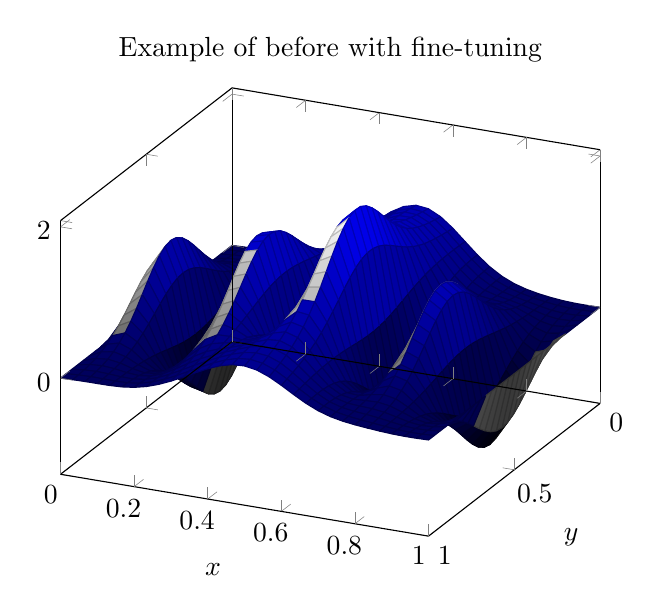
\begin{tikzpicture}
\begin{axis}[
    title=Example of before with fine-tuning,
    xlabel=$x$,
    ylabel=$y$,
]
    \addplot3 [
        surf,
        mesh/interior colormap={blueblack}{
            color=(black) color=(blue)
        },
        % slightly increase sampling quality (was 25):
        samples=31,
        % avoids overshooting corners:
        miter limit=1,
        % move boundary between inner and outer:
        mesh/interior colormap thresh=0.1,
        colormap/blackwhite,
        domain=0:1,
    ] {
        sin(deg(8*pi*x))* exp(-20*(y-0.5)^2)
            + exp(-(x-0.5)^2*30
                - (y-0.25)^2 - (x-0.5)*(y-0.25))
    };
\end{axis}
\end{tikzpicture}
\end{codeexample}
    %
    \noindent 这改善了显示效果。


    \paragraph{招募志愿者：}

    如果这些键的微调不是必需的，那就太好了。如果有人对如何改进此功能
    有充分依据的建议（例如知识或详尽的实验），请告诉我。

    注意，|mesh/interior colormap| 目前不能与 |mesh/refines| 组合。

    注意，|mesh/interior colormap| 由于法线向量的计算会增加编译时间。
\end{pgfplotskeylist}

\begin{pgfplotskey}{mesh/interior colormap thresh=\marg{Number between $-1.0$ and $+1.0$} (initially 0)}
    一个阈值，将 |colormap| 和 |interior colormap| 之间的边界向
    |colormap| 移动（如果值为负）或向 |interior colormap| 移动
    （如果值为正）。

    极端值 $-1$ 实质上停用 |interior colormap|，而另一个极端值 $+1$
    停用 |colormap|。

    示例见上文。
\end{pgfplotskey}
}

\begin{pgfplotskey}{surf shading/precision=\mchoice{pdf,postscript,ps} (initially postscript)}
    一个用于配置 |shader=interp| 的底层驱动如何写入其数据的键。选项
    |pdf| 使用 32~bit 二进制坐标（无损）。生成的 |.pdf| 文件看起来是
    正确的，但它们不能转换为 postscript——转换软件总是报错。

    选项 |postscript|（或简称 |ps|）使用 24~bit 截断的二进制坐标。
    这产生可读的 |.ps| 和 |.pdf| 文件。但是，截断是有损的。

    如果有人有如何修复此问题的想法：请告诉我。据我所知，Postscript
    应该接受 32~bit 坐标，所以这可能是着色驱动中的错误。
\end{pgfplotskey}


\subsection{带显式颜色的曲面图}

{
\tikzset{
    external/figure name/.add={}{surf_explicit_color_},
    /pdflinks/search key prefixes in/.add={}{,/pgfplots/mesh/},
}

\ref{sec:pgfplots:surfplots} 节中描述的曲面图都基于 |colormap|。本节
介绍一种不同类型的曲面图。实际上，它使用完全相同的 plot handlers：
适用于 |mesh|、|surf| 和 |patch| 图。但是，提供颜色的方式以及
\PGFPlots{} 插值颜色的方式有本质不同。

本节描述带显式颜色的曲面图。这些图为 |mesh| 的每个顶点期望如
|red|、|green| 或 |rgb=(0.5,0.2,1)| 这样的颜色——并在这些顶点之间
平滑插值。这似乎比基于 |colormap| 的曲面图更简单，也许更直接。其实
不然。带显式颜色的曲面图更难定义，也更难阅读。

如果你不确定应该使用由 |colormap| 着色的曲面还是显式颜色，基于下文
讨论的原因，你应该优先选择 |colormap|。

\begin{pgfplotskey}{mesh/color input=\mchoice{colormap,explicit,explicit mathparse} (initially colormap)}
    允许配置 \PGFPlots{} 如何期望曲面图的颜色输入。

    选项 \declaretext{colormap} 使用标准颜色图。此特定选项期望
    |point meta| 的标量值，这些值被线性映射到颜色图中。它类似于
    \ref{sec:pgfplots:surfplots} 节中更详细解释的曲面图。它是默认
    配置，（可能）涵盖最常见的用例。

    选项 \declaretext{explicit} 期望符号形式的显式提供的
    |point meta|：你的输入坐标流的每个坐标都应该有一个明确定义的
    颜色作为 |point meta|。这里，"显式提供"指的是
    |point meta=explicit symbolic|。此选项和可用的颜色格式在以下
    小节中详细解释。
    % (more precisely: in Section~\ref{sec:surf:explicit:color}).

    选项 \declaretext{explicit mathparse} 类似于 |explicit|，但它
    允许仅提供一个数学表达式，该表达式对每个坐标求值。数学表达式
    可以是 |rgb=x,y,0.5| 的形式，其中 |x| 用于定义"红"分量，|y|
    用于定义"绿"分量，"蓝"分量固定为 |0.5|。此键也在以下小节中
    更详细地解释。
    %, especially in Section~\ref{sec:surf:explicit:color:math}.
\end{pgfplotskey}

|mesh/color input=|\declaretext{colormap} 的主要用例是允许在插值颜色和
某些关注值之间建立映射。此映射可以显示为 |colorbar|：
%
% \usepgfplotslibrary{patchplots}
\begin{codeexample}[]
% \usepgfplotslibrary{patchplots}
\begin{tikzpicture}
\begin{axis}[small,view={0}{90},colorbar]
    \addplot3 [
        surf,
        shader=interp,
        patch type=bilinear,
    ] coordinates {
        (0,0,0) (1,0,0)

        (0,1,0) (1,1,1)
    };
\end{axis}
\end{tikzpicture}
\end{codeexample}
%
\noindent 注意，前面的示例是标准 |surf| 图，除了 |patch type=bilinear|，
后者控制颜色如何插值。有一个 $2 \times 2$ 矩阵，其 $z$ 值用作颜色
数据。显然，值 $z=0$ 对应蓝色，$z=1$ 对应红色——中间的所有其他颜色
与蓝色和红色没有直接关系；它们取自颜色图。颜色图定义出现哪些颜色：
构成颜色图的颜色以及可以作为颜色图颜色之间的插值颜色出现的颜色。
颜色的成对混合是 |mesh/color input=colormap| 的属性，而不是
|mesh/color input=explicit| 的属性（后者混合两种以上的颜色）。
此外，曲面指示恒定 $z$ 水平的等高线。以黄色等高线为例。我们知道它
有某个介于 $0.3$ 和 $0.4$ 之间的值，比如 $0.35$。由于这些着色是
连续的，我们知道点 $z=0.35$ 出现在 $z=0$ 和 $z=1$ 之间——在曲面的
每个点处。由于颜色图，曲面上具有 $z=0.35$ 的每个点将获得黄色。这是
因为插值是对标量 |point meta| 值执行的，然后映射到 |colormap| 中。
这种等高线属性也是颜色图曲面独有的。

其他两个选项在下一小节中详细解释。


\subsubsection{为每个坐标显式提供颜色}
\label{sec:surf:explicit:color}

以下是一个简单的方法，与上面颜色图示例具有相同的顶点，但使用显式
颜色：
%
% \usepgfplotslibrary{patchplots}
\begin{codeexample}[]
% \usepgfplotslibrary{patchplots}
\begin{tikzpicture}
\begin{axis}[small,view={0}{90}]
    \addplot3 [
        surf,
        shader=interp,
        patch type=bilinear,
        mesh/color input=explicit,
    ] coordinates {
        (0,0,0) [color=blue]   (1,0,0) [color=green]

        (0,1,0) [color=yellow] (1,1,1) [color=red]
    };
\end{axis}
\end{tikzpicture}
\end{codeexample}
%
\noindent 坐标和视图是相同的，甚至颜色
双线性插值的方式也相同。但是，我们在
角点处有四种不同的颜色。我们在输出中看到这些角点，并且看到它们被平滑地
混合在一起。然而，混合包含所有四种颜色，而不仅仅是两种。因此
直接的结果是，没有等高线。

缺乏如何将颜色信息映射到"数据可视化的某些信息"的直接信息，这意味着
\emph{如果}你想使用带显式颜色的 |surf|ace 图，你必须清楚地说明你
想显示什么。这对于 |colormap| 来说要简单得多。

以下示例配置 $z=0$ 接收 |blue|，$z=1$ 接收
|red|，如同我们前面的 |colormap| 示例（见上文）一样，使用
|mesh/color input=|\declaretext{explicit}。
%
% \usepgfplotslibrary{patchplots}
\begin{codeexample}[]
% \usepgfplotslibrary{patchplots}
\begin{tikzpicture}
\begin{axis}[small,view={0}{90}]
    \addplot3 [
        surf,
        shader=interp,
        patch type=bilinear,
        mesh/color input=explicit,
    ] coordinates {
        (0,0,0) [color=blue] (1,0,0) [color=blue]

        (0,1,0) [color=blue] (1,1,1) [color=red]
    };
\end{axis}
\end{tikzpicture}
\end{codeexample}
%
\noindent 我们看到插值的双线性性质；它与上面的
|mesh/color input=colormap| 有关（比较中间的等高线）。在大多数情况下，
你只是想展示一些等高线。对于这种情况，|colormap| 是正确的选择。

可能存在 |mesh/color input=explicit| 适用的情况。但是，你需要仔细思考。
并且你需要清楚地解释你做了什么，因为你的受众在理解任何基于显式颜色
插值的数据可视化之前也需要大量思考。

选项 |mesh/color input=explicit| 期望产生符号值的 |point meta| 选择。
在这种上下文中，"符号"指的是一种特殊的颜色定义：
%
\begin{codeexample}[]
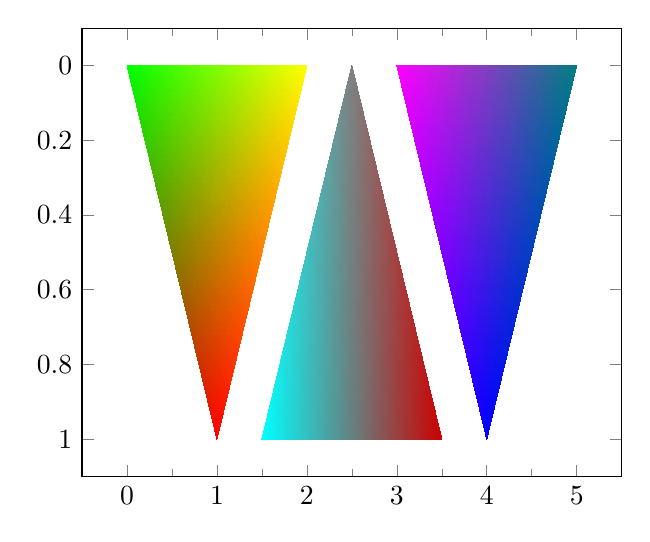
\begin{tikzpicture}
\begin{axis}[minor x tick num=1]
    \addplot [
        patch,
        shader=interp,
        mesh/color input=explicit,
    ] table [meta=c] {
        x y c
        0 0 color=green
    % default color model is rgb:
        1 1 1,0,0
        2 0 1,1,0

        1.5 1 cmyk=1,0,0,0
        2.5 0 gray=0.5
        3.5 1 color=red!80!black

        3 0 1,0,1
        4 1 0,0,1
        5 0 rgb255=0,128,128
    };
\end{axis}
\end{tikzpicture}
\end{codeexample}
%
\noindent 前面的示例定义了一个 |patch| 图，包含三个三角形补丁，每个
由三个顶点组成，这些顶点按原样放入输入坐标流。每个顶点在列 |c| 中
有其颜色数据。颜色规范的格式在下一段中更详细地解释。

一旦你写入 |mesh/color input=explicit|，\PGFPlots{} 会检查
|point meta| 的当前值。如果 |point meta| 的当前值是 |none|，它被
设置为 |point meta=explicit symbolic|（这就是我们上面示例中发生的
情况）。如果 |point meta| 的当前值是产生数字输出的某个选项（如
|point meta=x| 或 |point meta=\thisrow{x}+1|），它被设置为
|point meta=explicit symbolic|。如果 |point meta| 的当前值已经是
符号形式，则保持不变。

因此，我们上面的示例在遇到 |mesh/color input=explicit| 时设置
|point meta=explicit symbolic|。显式符号输入处理器反过来期望坐标流
为每个流式坐标提供点元数据。我们在这里使用表，表从 |table/meta|
键中提供的列名读取其颜色数据。

接受的颜色格式与颜色图定义的格式非常相似（比较
\pageref{sec:colormap:input:format} 页的
\ref{sec:colormap:input:format} 节）。通用格式是
\declaretext{\meta{color model}|=|\meta{arguments}}。与颜色图定义内
类似的输入格式相比，这里的语法没有圆括号，也没有 \meta{length}
参数。尽管如此，接受相同的 \meta{color model} 和相同的
\meta{arguments}。选项有
%
% ATTENTION : a VERY similar description (actually: the same) is in the
% colormap section
% maintain both; the syntax is different
\begin{description}
        \renewcommand\makelabel[1]{\declaretext{#1}}%
        \setlength{\labelsep}{0pt}
    \item[rgb] |=|\meta{red}|,|\meta{green}|,|\meta{blue} 其中每个
        分量在区间 $[0,1]$ 内，
    \item[rgb255] |=|\meta{red}|,|\meta{green}|,|\meta{blue} 与
        |rgb| 类似，除了每个分量期望在区间 |[0,255]| 内，
    \item[gray] |=|\meta{value} 其中 \meta{value} 在区间 $[0,1]$ 内，
    \item[color] |=|\meta{named color} 其中 \meta{named color} 是
        预定义（命名）颜色如 `|red|' 或颜色表达式如 `|red!50|'，
    \item[cmyk]
        |=|\meta{cyan}|,|\meta{magenta}|,|\meta{yellow}|,|\meta{black} 其中
        每个分量在区间 $[0,1]$ 内，
    \item[cmyk255]
        |=|\meta{cyan}|,|\meta{magenta}|,|\meta{yellow}|,|\meta{black} 与
        |cmyk| 相同，但期望分量在区间 $[0,255]$ 内，
    \item[cmy] |=|\meta{cyan}|,|\meta{magenta}|,|\meta{yellow} 其中每个
        分量在区间 $[0,1]$ 内，
    \item[hsb] |=|\meta{hue}|,|\meta{saturation}|,|\meta{brightness} 其中
        每个分量在区间 $[0,1]$ 内，
    \item[Hsb] |=|\meta{hue}|,|\meta{saturation}|,|\meta{brightness} 与
        |hsb| 相同，除了 \meta{hue} 接受区间 $[0,360]$ 内的值（度），
    \item[HTML] |=|\meta{hex red}\meta{hex green}\meta{hex blue} 其中
        分量期望是介于 |00| 和 |FF| 之间的十六进制数（|rgb255| 的
        变体），
    \item[wave] |=|\meta{wave length} 期望单个波长作为数值参数，
        范围 $[363,814]$。
\end{description}


\begin{pgfplotskey}{mesh/colorspace explicit color input=\allowbreak\mchoice{%
        rgb,rgb255,
        cmy,
        cmyk,cmyk255,
        gray,
        wave,
        hsb\\,Hsb,
        HTML%
    } (initially rgb)%
}
    如果输入颜色\emph{没有颜色模型}，颜色分量被解释为作为此键参数
    指定的颜色模型中的颜色。

    此键只有一个目的：当 \meta{color model} 对许多点都相同时，省略
    它。
\end{pgfplotskey}

\begin{pgfplotskey}{%
    mesh/colorspace explicit color output=\mchoice{rgb,cmyk,gray} (initially rgb)%
}
    调查阶段遇到的任何颜色（即在检查 |point meta| 值时）立即被转换为
    配置为 |mesh/colorspace explicit color output| 的颜色空间。

    注意，如果你告诉 |xcolor| 全局覆盖颜色空间，此选项\emph{无效}。
    更确切地说，使用
    %
\begin{codeexample}[code only]
\usepackage[cmyk]{xcolor}
\end{codeexample}
    %
    或者，
    %
\begin{codeexample}[code only]
\selectcolormodel{cmyk}
\end{codeexample}
    %
    将导致所有颜色转换为 |cmyk|，\PGFPlots{} 遵循此配置。因此，这两个
    语句都导致所有颜色在期望的颜色空间中插值，并且所有输出颜色将
    使用此颜色空间。这通常正是你需要的。

    转换后的颜色用于任何颜色插值。在大多数情况下，这由 |shader| 完成，
    但它也适用于 |patch refines| 和 |patch to triangles|。

    由于转换后的颜色用于颜色插值，可用的\emph{输出}颜色空间列表比
    可用的\emph{输入}颜色空间小得多。只有设备颜色空间
    \declaretext{rgb}、\declaretext{gray} 和 \declaretext{cmyk} 可用
    作 |mesh/colorspace explicit color output| 的值。

    任何必要的颜色空间转换依赖于 |xcolor|
    包。\footnote{颜色空间转换对于 plain \TeX{} 和 Con\TeX{}t 不可用。
    对于这些情况，你必须确保输入和输出颜色模型相同。} 注意，颜色空间
    转换受最近颜色匹配的约束，即它们不太精确。这通常远远超出纯舍入
    问题；它是由这些颜色空间实际上如此不同以至于转换难以完成这一
    事实引起的。如果你能在正确的颜色空间中立即指定颜色，你可以消除
    此类转换。

    以下是相同的着色，一次使用 CMYK 输出，一次使用 RGB 输出。根据
    你的输出介质（屏幕或纸张），在比较图片时你会观察到略有不同的
    颜色。
    %
\begin{codeexample}[]
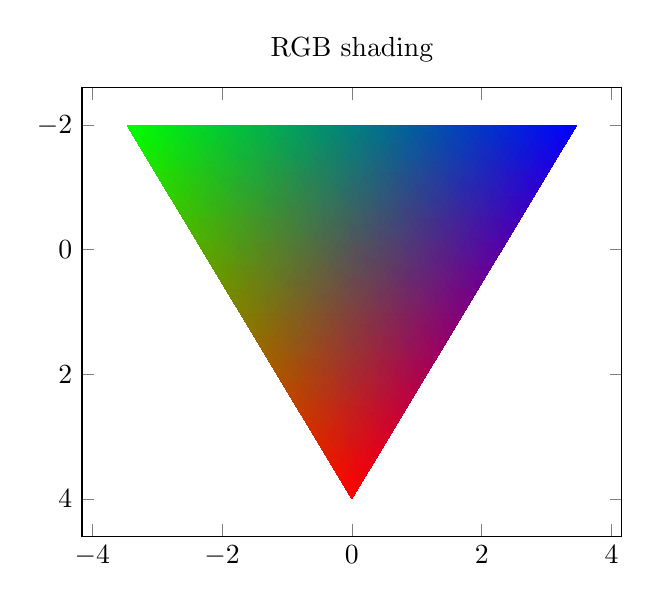
\begin{tikzpicture}
\begin{axis}[title=RGB shading]
    \addplot [
        patch,
        shader=interp,
        mesh/color input=explicit,
        mesh/colorspace explicit color output=rgb,
        data cs=polar,
    ] coordinates {
        (90,4)  [color=red]
        (210,4) [color=green]
        (-30,4) [color=blue]
    };
\end{axis}
\end{tikzpicture}
\end{codeexample}

\begin{codeexample}[]
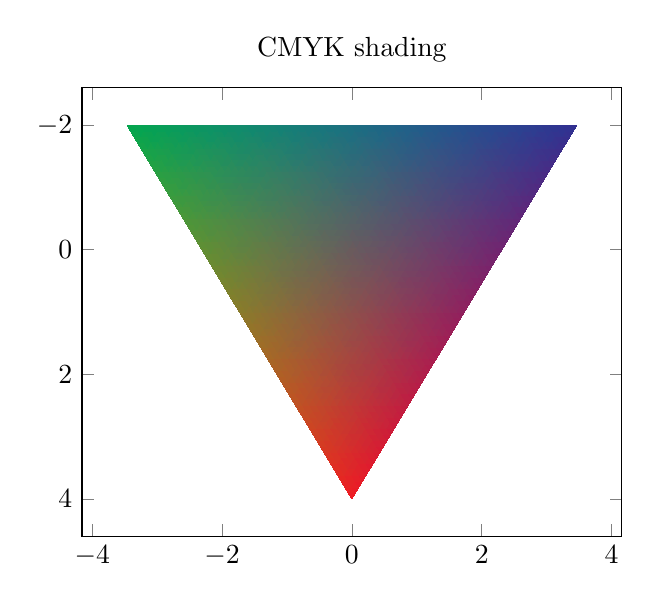
\begin{tikzpicture}
\begin{axis}[title=CMYK shading]
    \addplot [
        patch,
        shader=interp,
        mesh/color input=explicit,
        mesh/colorspace explicit color output=cmyk,
        data cs=polar,
    ]
    coordinates {
        (90,4)  [color=red]
        (210,4) [color=green]
        (-30,4) [color=blue]
    };
\end{axis}
\end{tikzpicture}
\end{codeexample}

    此键与相关键 |colormap default colorspace| 类似，尽管值可以独立
    选择。
\end{pgfplotskey}


\subsubsection{将颜色分量作为表提供}

上一节展示了如何为每个坐标提供单个符号颜色表达式，即使用
|point meta=explicit symbolic|。

另一个用例可能是提供一个包含坐标值和按颜色分量分列的表。为了从输入
表组装颜色规范，你可以提供符号表达式：
%
\begin{codeexample}[]
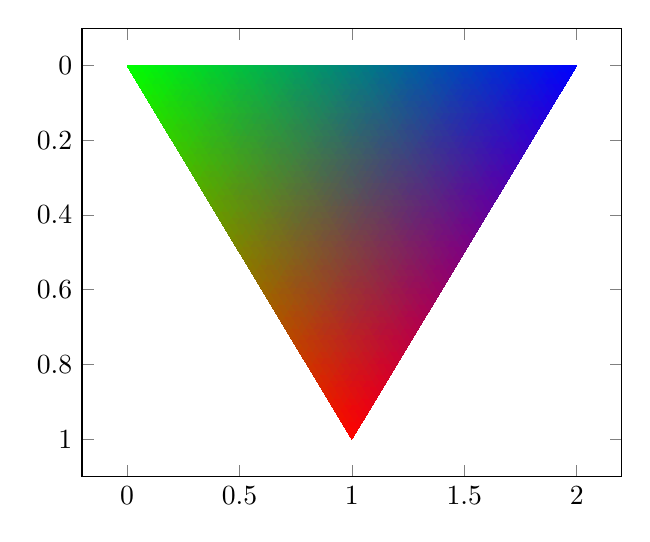
\begin{tikzpicture}
\begin{axis}
    \addplot [
        patch,
        shader=interp,
        mesh/color input=explicit,
        point meta={symbolic=
            {\thisrow{R},\thisrow{G},\thisrow{B}}
        },
    ] table {
        x y R G B
        0 0 0 1 0
        1 1 1 0 0
        2 0 0 0 1
    };
\end{axis}
\end{tikzpicture}
\end{codeexample}
%
前面的示例使用了带三角形元素的 |patch| 图，正如我们之前看到的。
此外，它使用显式颜色输入——但与 |point meta={symbolic=|\marg{value}|}|
结合（注意额外的一对花括号）。此选择接受输入上的任意符号，这些符号
将被重新评估
（展开）用于每个坐标。在我们的示例中，我们只是使用 |\thisrow| 从
表格列中读取值。由于默认的输入颜色空间是 RGB，这
会得到预期的具有红、绿、蓝角点的三角形。结果
必须构成有效的颜色规范。

注意，在这种上下文中，符号表达式纯粹是基于字符串的。如果你计划
使用数学表达式，必须使用 |mesh/color input=explicit mathparse|，
如下一节所述。


\subsubsection{将颜色作为数学表达式提供}
\label{sec:surf:explicit:color:math}

键 |mesh/color input| 有两个用于显式颜色输入的选项。选项
\declaretext{explicit} 已在前面的段落中讨论，它为每个需要颜色的节点
期望一个颜色规范。它还接受一种基于字符串的表达式，以合适的方式拼接
期望的颜色规范。

第二个选项 |mesh/color input=|\declaretext{explicit mathparse} 几乎
相同——但有一个主要区别：它允许在 |point meta| 值内部提供数学表达式。
但是，提供的数学表达式需要形成一个通常具有多个颜色分量的颜色规范。

使用此选项时，|point meta| 的值是符号形式，但颜色分量由数学解析器
对每个具有颜色数据的输入点重新求值。提供此类表达式最方便的方式是
|point meta={symbolic={|\meta{R},\meta{G},\meta{B}|}}|（再次注意参数
的额外大括号）。

\begin{codeexample}[]
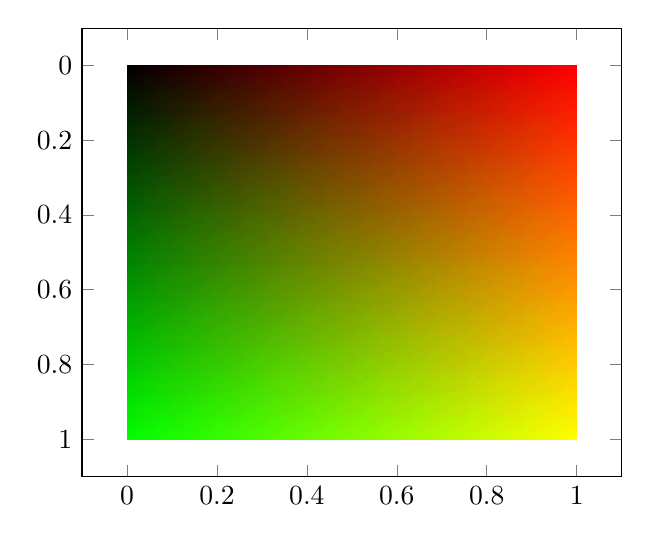
\begin{tikzpicture}
\begin{axis}
    \addplot [
        surf,
        shader=interp,
        mesh/color input=explicit mathparse,
        point meta={symbolic={x,\thisrow{y},0}},
    ] table {
        x y
        0 0
        1 0

        0 1
        1 1
    };
\end{axis}
\end{tikzpicture}
\end{codeexample}
%
\noindent 前面的示例是一个带有 $2 \times 2$ 输入矩阵的 |surf|ace 图。
注意，该表没有显式点元数据。|point meta| 数据从一个通用数学表达式
获取，该表达式使用最终 $x$ 坐标作为 \meta{red} 分量，当前行和列
|y| 中看到的值作为 \meta{green} 值，常量值 \meta{blue}$=0$。
因此，输出在左下角是黑色，因为黑色是 $(0,0,0)$，在右下角是红色，
在左上角是绿色，沿对角线是两者的混合。

作为 |point meta={symbolic=|\marg{value}|}| 提供的值与
|mesh/color input=explicit| 的形式相同，即它应该是
\meta{color model}|=|\meta{color components} 的形式。如果省略
\meta{color model}，它默认为 |mesh/colorspace explicit color input|
（默认为 |rgb|）。

由于数学表达式可以是任意的，它可以安全地与表达式绘图结合使用。

一个潜在用例可能是展示一个具有 $(x,y,z)$ 的曲面和一些二维量，该量
被编码为红色和绿色的混合。以下示例依赖
|mesh/color input=|\declareandlabel{explicit mathparse} 和
|point meta=symbolic| 来提供数学表达式向量：
%
\pgfplotsexpensiveexample
% \usepgfplotslibrary{patchplots}
\begin{codeexample}[]
% \usepgfplotslibrary{patchplots}
\begin{tikzpicture}
\begin{axis}
% this example burns colors if opacity
% is active in the document.
    \addplot3 [
        patch,
        patch type=bilinear,
        mesh/color input=explicit mathparse,
        domain=0:1,
        samples=30,
        point meta={
            symbolic={
                (sin(deg(x*pi*2))+1)/2, % R
                (sin(deg(y*pi*2))+1)/2, % G
                0                       % B
            }
        },
    ] {sin(deg(x*pi*2))+sin(deg(y*pi*2))};
\end{axis}
\end{tikzpicture}
\end{codeexample}
%
\noindent 注意，前面的示例存在\index{color burning}
颜色灼烧问题：\footnote{至少在 Acrobat Reader 中。} 绿色区域变得
太亮，黑色区域变得太暗。注意，如果图片作为独立图片写出，它是完全
可接受的。但是，一旦你将图片（作为 |.pdf| 或 |.png|）导入到启用了
|opacity| 的文档中，它就会出现颜色灼烧。

颜色灼烧是由 RGB 颜色空间、此示例中设置的特殊颜色以及由 |opacity|
激活的颜色混合共同引起的。注意，只需在文档某处激活 |opacity|
即可。

为了修复当前图片的问题，必须选择不同的输出颜色空间：

\pgfplotsexpensiveexample
% \usepgfplotslibrary{patchplots}
\begin{codeexample}[]
% \usepgfplotslibrary{patchplots}
\begin{tikzpicture}
\begin{axis}
    \addplot3 [
        patch,
        patch type=bilinear,
        mesh/color input=explicit mathparse,
        %
        % CMYK produces better quality here
        % since the manual has opacity enabled
        mesh/colorspace explicit color output=cmyk,
        domain=0:1,
        samples=30,
        point meta={
            symbolic={
                (sin(deg(x*pi*2))+1)/2, % R
                (sin(deg(y*pi*2))+1)/2, % G
                0                       % B
            }
        },
    ] {sin(deg(x*pi*2))+sin(deg(y*pi*2))};
\end{axis}
\end{tikzpicture}
\end{codeexample}
%
\noindent 键 |mesh/colorspace explicit color output| 将每个输入 RGB
颜色转换为匹配的 CMYK 颜色。这反过来是一种有损转换，似乎没有简单的
解决方案。\footnote{如果某些颜色空间操作专家能在此贡献最佳实践，
请随时联系我。}

数学表达式也可用于复杂的输入颜色空间，例如 |wave| 颜色空间。
%
\begin{codeexample}[]
\begin{tikzpicture}
\begin{axis}
    \addplot3 [
        surf,
        shader=interp,
        mesh/color input=explicit mathparse,
        domain=0:1,
        samples y=2,
        point meta={symbolic={wave=363+x*(814-363)}},
    ] {x*y};
\end{axis}
\end{tikzpicture}
\end{codeexample}

注意，你必须注意颜色分量在期望的范围内。
}%


\subsection{等高线图}
{
\pgfkeys{
    /pdflinks/search key prefixes in/.add={}{,/pgfplots/contour/,/pgfplots/contour external/},
    /pgfmanual/gray key prefixes/.add={/pgfplots/contour/,}{},
}%
\tikzset{external/figure name/.add={}{contour_}}%
%
\PGFPlots{} 支持等高线图的可视化。由于这些算法的复杂性，
\PGFPlots{} 需要更多计算能力。你可以在 |contour lua|（不需要安装
额外软件，但需要调用 |lualatex| 而不是 |pdflatex|）和
|contour gnuplot|（需要允许 \TeX{} 调用 |gnuplot| 并安装
|gnuplot|）之间选择。

|contour lua| 和 |contour gnuplot| 都期望与 |mesh| 或 |surf| 相同
格式的矩阵输入（包括任何 \PGFPlots{} 矩阵输入方法）。在撰写本文时，
两者都需要临时文件用于输入和输出数据。生成的等高线使用
|contour prepared| plot handler 可视化，该 handler 接受预计算的
等高线坐标并处理其可视化（|contour/draw color|、|contour/labels|
等）。简而言之：两个 plot handler 都期望通常的矩阵输入并生成等高线。
推荐的可视化等高线方式是 |contour lua|，因为它不需要第三方程序，
但需要调用 |lualatex|。

我们首先讨论外部程序的高层接口，稍后继续讨论 |contour prepared|。

\begin{plottype}[/pgfplots]{
    contour lua=\textcolor{black}{\marg{{\normalfont options with
    `\texttt{contour/}' or `\texttt{contour external/}' prefix}}}%
}
{\emph{此算法由 Francesco Poli 实现并贡献}}

    这是一个高层等高线图接口。它以与二维 |surf| 或 |mesh| 图相同的
    方式期望矩阵数据。然后它计算等高线并可视化它们。
    %
\pgfplotsexpensiveexample
\begin{codeexample}[]
\begin{tikzpicture}
\begin{axis}[view={0}{90}]
    \addplot3 [
        contour lua
    ] {x*y};
\end{axis}
\end{tikzpicture}
\end{codeexample}
    %
    \noindent 该示例使用 \verbpdfref{\addplot3} 以及 |expression|
    绘图，这意味着输入数据的形式为 $(x_i,y_i,f(x_i,y_i))$。
    |view={0}{90}| 标志意味着"从顶部查看"，否则等高线将被绘制为
    $z$ 值：
%
\pgfplotsexpensiveexample
\begin{codeexample}[]
\begin{tikzpicture}
\begin{axis}
    \addplot3 [
        contour lua
    ] {exp(0-x^2-y^2)};
\end{axis}
\end{tikzpicture}
\end{codeexample}

    如前所述，你可以使用任何 \PGFPlots{} 输入方法，只要它产生矩阵
    输出。因此，我们可以重用矩阵数据的介绍性示例，这次使用内联
    数据：
    %
\pgfplotsexpensiveexample
\begin{codeexample}[]
\begin{tikzpicture}
\begin{axis}[view={0}{90}]
    \addplot3 [
        contour lua
    ] coordinates {
        (0,0,0) (1,0,0)   (2,0,0)   (3,0,0)

        (0,1,0) (1,1,0.6) (2,1,0.7) (3,1,0.5)

        (0,2,0) (1,2,0.7) (2,2,0.8) (3,2,0.5)
    };
\end{axis}
\end{tikzpicture}
\end{codeexample}
    %
    \noindent 幕后发生的事情是，\PGFPlots{} 接受输入矩阵并将所有
    遇到的坐标写入临时文件，包括扫描线结束标记。然后，它生成一个
    小的 |lua| 脚本并调用 |lua| 算法计算等高线坐标，将所有内容写入
    临时输出文件。之后，它包含 |lua| 的输出文件，就像你写入
    |\addplot3[contour prepared] file |\marg{temporaryfile}|;| 一样。

    所有这些 |lua| 调用，包括输入/输出文件管理，对用户是透明的。
    它只需要两件事：首先，它需要矩阵数据作为输入。\footnote{注意，
    \texttt{contour lua} 仅处理输入流一次。因此，临时文件将仅包含
    在第一个点被看到之前可用的信息。上面的示例有效，因为它包含
    |empty line| 作为扫描线结束标记。如果你不提供此类标记，你可能
    需要提供三个选项 \texttt{mesh/rows}、\texttt{mesh/cols} 或
    \texttt{mesh/num points} 中的两个。}

    |contour lua| 的等高线算法接受 $(x,y,z)$ 以及 |point meta|。
    其等高线信息始终基于 |point meta|。通常，|point meta| 和 $z$
    相同。但也可以使用不同的 |point meta|：

\begin{codeexample}[]
\begin{tikzpicture}
\begin{axis}[
	xlabel={$x$}, ylabel={$y$}, zlabel={$z$},
	view/h=70,
	view/v=50,
]
% z= -x+y
\addplot3[surf,samples=2,shader=interp]
table {
  x       y       z
  -5      -5      0
   5      -5      -10

  -5       5      10
   5       5      0
};

% same data, but with contour
% and color data v= x+y :
\addplot3[
  contour lua={number=3},
  point meta=\thisrow{v},
]
table {
  x       y       z         v
  -5      -5      0        -10
   5      -5      -10      0

  -5       5      10       0
   5       5      0        10
};
\end{axis}
\end{tikzpicture}
\end{codeexample}

    结果数据可以投影到单独的切片上，例如使用 |z filter|。
    %
\pgfplotsexpensiveexample
\begin{codeexample}[]
\begin{tikzpicture}
\begin{axis}
    \addplot3 [
        surf,
        shader=interp
    ] coordinates {
        (0,0,0) (1,0,0)   (2,0,0)   (3,0,0)

        (0,1,0) (1,1,0.6) (2,1,0.7) (3,1,0.5)

        (0,2,0) (1,2,0.7) (2,2,0.8) (3,2,0.5)
    };
    \addplot3 [
        contour lua,
        z filter/.code={\def\pgfmathresult{1}},
    ] coordinates {
        (0,0,0) (1,0,0)   (2,0,0)   (3,0,0)

        (0,1,0) (1,1,0.6) (2,1,0.7) (3,1,0.5)

        (0,2,0) (1,2,0.7) (2,2,0.8) (3,2,0.5)
    };
\end{axis}
\end{tikzpicture}
\end{codeexample}

    输入/输出文件管理有几个微调参数，甚至可以调用不同于 |lua| 的
    程序（参见 |contour gnuplot|）。这些细节在本节末尾讨论，参见下文
    \pageref{key:pgfplots:contour:gnuplot} 页。
\end{plottype}

\begin{pgfplotskey}{contour/number=\marg{integer} (initially 5)}
    配置任何等高线算法应生成的等高线数量。该值同时应用于
    |contour lua| 和 |contour filled|。
    %
\pgfplotsexpensiveexample
\begin{codeexample}[]
\begin{tikzpicture}
\begin{axis}[
    title={$x \exp(-x^2-y^2)$},
    domain=-2:2,enlarge x limits,
    view={0}{90},
]
    \addplot3 [
        contour lua={number=14, labels=false},
        thick,
    ] {exp(-x^2-y^2)*x};
\end{axis}
\end{tikzpicture}
\end{codeexample}
    %
    也可以更改 |/pgf/number format| 设置，参见下文
    |contour/every contour label| 样式的文档。

    注意，|contour/number| 对 |contour prepared| 无效。
\end{pgfplotskey}

\begin{pgfplotskey}{contour/levels=\marg{list of levels} (initially empty)}
    通过离散层级列表配置任何等高线算法应生成的等高线数量。
    %
\pgfplotsexpensiveexample
\begin{codeexample}[]
\begin{tikzpicture}
\begin{axis}[
    title={$x \exp(-x^2-y^2)$},
    domain=-2:2,
    enlargelimits,
    view={0}{90},
]
    \addplot3 [
         contour lua={levels={-0.1,-0.2,-0.6}},
         thick,
    ] {exp(-x^2-y^2)*x};
\end{axis}
\end{tikzpicture}
\end{codeexample}
    %
    也可以更改 |/pgf/number format| 设置，参见下文
    |contour/every contour label| 样式的文档。

    此键优先级高于 |contour/number|，即如果两者都给出，
    |contour/levels| 将生效。

    注意，|contour/levels| 对 |contour prepared| 无效。
\end{pgfplotskey}

\begin{pgfplotskey}{contour/contour dir=\mchoice{x,y,z} (initially z)}
        \tikzset{external/figure name/.add={}{contourdir_}}%
	\paragraph{注意：} 引入键 |contour dir| 是为了支持在三个坐标上操作的外部等高线算法（如 |contour gnuplot|）。但是，|contour lua| 在 $(x,y,z)$ 和 |point meta| 上操作，可以使用 |point meta=x| 达到相同效果！因此，自从 |contour lua| 出现以来，此键的重要性已降低。

    此键允许相对于另一个方向生成等高线。
    %
\pgfplotsexpensiveexample
\begin{codeexample}[]
\begin{tikzpicture}
\begin{axis}[
    title={$x \exp(-x^2-y^2)$},
    domain=-2:2,
]
    \addplot3 [
        contour lua={
            contour dir=x,
            labels=false,
            number=15,
        },
        thick,
    ] {exp(-x^2-y^2)*x};
\end{axis}
\end{tikzpicture}
\end{codeexample}


    输入数据与之前相同——必须以矩阵形式给出。键 |contour dir|
    配置算法沿提供的方向计算等高线。

\pgfplotsexpensiveexample
\begin{codeexample}[]
\begin{tikzpicture}
\begin{axis}[
    title={$x \exp(-x^2-y^2)$},
    domain=-2:2,
]
    \addplot3 [
        contour lua={
            contour dir=y,
            labels=false,
            number=15,
        },
        thick,
    ] {exp(-x^2-y^2)*x};
\end{axis}
\end{tikzpicture}
\end{codeexample}

    此功能也可用于参数化曲面。

\pgfplotsexpensiveexample
\begin{codeexample}[]
\begin{tikzpicture}
\begin{axis}[view={60}{30},axis equal image]
    \addplot3 [
        contour lua={
            contour dir=x,
            number=20,
            labels=false,
        },
        samples=30,domain=-1:1,y domain=0:2*pi,
    ] (
        {sqrt(1-x^2) * cos(deg(y))},
        {sqrt( 1-x^2 ) * sin(deg(y))},
         x
    );
\end{axis}
\end{tikzpicture}
\end{codeexample}

    但是注意，每条等高线接收单一颜色。这是等高线图所期望的：它有
    单一的样式和单一的等高线层级。此外注意，分配给 |contour dir=x|
    的等高线图的颜色与分配给 |contour dir=z| 的等高线图的颜色
    \emph{不同}：|contour dir| 的参数隐式定义了 |point meta| 的
    参数（也称为颜色数据）。更确切地说，|contour dir=x| 的等高线图
    具有 |point meta=x|，而 |contour dir=z| 的等高线图使用
    |point meta=z|。

    如果你希望等高线内部有单独着色的段，你必须使用不同的 plot
    handler。有一个简单的替代方案在许多情况下效果良好：你可以使用
    标准 |mesh| 图结合 |patch type=line|：

\pgfplotsexpensiveexample
\begin{codeexample}[]
\begin{tikzpicture}
\begin{axis}[
    title={$x \exp(-x^2-y^2)$},
    domain=-2:2,
    xlabel=$x$, ylabel=$y$,
]
    \addplot3 [
        samples y=10,
        samples=25,
        mesh,
        patch type=line,
        thick,
    ] {exp(-x^2-y^2)*x};
\end{axis}
\end{tikzpicture}
\end{codeexample}

    这里，我们\emph{没有}生成等高线图。我们生成了一个带有
    |patch type=line| 的 |mesh| 图。选项 |patch type=line| 产生
    本质上一维的图，与 |mesh| 在不同情况下生成的默认矩阵样式
    可视化相反。\index{mesh!scanlinewise}\index{mesh!patch type=line}
    由于网格图为每个补丁段使用一种颜色，我们有很大的自由度来为
    段着色。在上面的示例中，我们使用默认配置 |point meta=z|，
    即 $z$ 值定义颜色。

    带有 |patch type=line| 的 |mesh| 图产生与 |contour dir=y|
    几乎相同的输出，这是扫描线编码的产物。我们的示例使用
    依赖于 |mesh/ordering=x varies| 的 |\addplot3 expression|。
    如果我们通过 |patch type=line| 可视化生成的矩阵，可视化遵循
    沿 $x$ 轴变化的扫描线。在我们的示例中，我们使用
    |samples y=10| 来控制"等高线"的数量。

    上一段的结果是，如果我们想获得与 |contour dir=x| 相同的效果，
    我们面临更具挑战性的任务：我们需要 |mesh/ordering=y varies|。
    在我们的情况下，我们需要转置数据矩阵。对于
    |\addplot3 expression|，这相对简单：我们可以交换 |x| 和 |y|
    的含义来获得转置：

\pgfplotsexpensiveexample
\begin{codeexample}[]
\begin{tikzpicture}
\begin{axis}[
    title={$x \exp(-x^2-y^2)$},
    domain=-2:2,
    xlabel=$x$,
    ylabel=$y$,
]
    \addplot3 [
        samples y=10,
        samples=25,
        mesh,
        patch type=line,
        thick,
    ] (y,x,{exp(-x^2-y^2)*y});
\end{axis}
\end{tikzpicture}
\end{codeexample}
    %
    这与上面的示例相同——但如你所注意到的，表达式中 |x| 和 |y|
    的含义已交换，并且符号已切换为参数图。这种方法也适用于数据
    文件，但 \PGFPlots{} 不能自行转置矩阵排序。


    回到 |contour dir|，我们还可以使用其输出来生成多个等高线投影，
    使用坐标过滤器。
    %
\pgfplotsexpensiveexample
\begin{codeexample}[]
\begin{tikzpicture}
\begin{axis}[
    xlabel=$x$,ylabel=$y$,
    enlargelimits=false,
    3d box=complete,
]
    \addplot3 [surf] {x^2-y^2};

    \addplot3 [
        contour lua={contour dir=y,
            draw color=red,labels=false},
        y filter/.expression={-5},
    ] {x^2-y^2};

    \addplot3 [
        contour lua={contour dir=x,
            draw color=blue,labels=false},
        x filter/.expression={5},
    ] {x^2-y^2};

    \addplot3 [
        contour lua={contour dir=z,
            draw color=black,labels=false},
        z filter/.expression={25},
    ] {x^2-y^2};
\end{axis}
\end{tikzpicture}
\end{codeexample}
    %
    \noindent 前面的示例使用固定的 |draw color| 结合 |x filter|、
    |y filter| 和 |z filter| 将等高线固定在其中一个坐标轴平面中。


    \paragraph{技术背景：}

    本节可能不必要，可以跳过。键 |contour dir| 通过坐标置换实现。
    由于等高线算法始终支持 |contour dir=z|，从输入矩阵 $X, Y, Z$
    计算 $z$--等高线相对简单。选项 |contour dir=z| 键直接按原样
    接受输入。选项 |contour dir=x| 将输入坐标重排为 |yzx|。选项
    |contour dir=y| 将输入坐标重排为 |xzy|。所有这些重排在坐标
    移交给等高线算法（参见 |contour external|）之前应用，并在从
    等高线算法读回结果时撤销。这意味着 |contour dir| 也可用于
    |contour prepared|。在此上下文中，|contour prepared| 应该是
    某个等高线算法的输出。其输入坐标根据逆置换自动重排。这允许
    绘制以准备格式给出的 $x$ 或 $y$ 等高线。
\end{pgfplotskey}

\begin{plottype}[/pgfplots]{
    contour gnuplot=\textcolor{black}{\marg{{\normalfont options with
    `\texttt{contour/}' or `\texttt{contour external/}' prefix}}}%
}
    这是一个高层等高线图接口。它以与二维 |surf| 或 |mesh| 图相同
    的方式期望矩阵数据。然后它计算等高线并可视化它们。handler
    |contour gnuplot| 的工作方式与 |contour lua| 完全相同，产生
    质量可比较的结果。上面提到的所有键和示例也适用于
    |contour gnuplot|。但是，在使用 |contour gnuplot| 之前，你必须
    应用以下步骤：
\begin{enumerate}
	\item install |gnuplot| on your system.
	\item Ensure that you can invoke |gnuplot| from a terminal (like cmd.exe or bash). To this end, you will need to add |gnuplot| to the PATH environment variable.
	\item When invoking |pdflatex|, you need to enable system calls.

        对于 \TeX{}Live，这是 |pdflatex -shell-escape|。对于 MiK\TeX{}，系统使用 |pdflatex -enable-write18|。某些 \TeX\ 发行版要求你为该选项使用两个斜杠。
\end{enumerate}
	另请参阅 \verbpdfref{plot gnuplot} 的文档以了解相关章节。



	用法与 |contour lua| 相同，因此请参阅 |contour lua| 及其示例。

    %
\pgfplotsexpensiveexample
\begin{codeexample}[]
\begin{tikzpicture}
\begin{axis}[view={0}{90}]
    \addplot3 [
        contour gnuplot
    ] {x*y};
\end{axis}
\end{tikzpicture}
\end{codeexample}

\pgfplotsexpensiveexample
\begin{codeexample}[]
\begin{tikzpicture}
\begin{axis}[view={0}{90}]
	\addplot3 [
		contour gnuplot={number=6}
	] {exp(-x^2-y^2)};
\end{axis}
\end{tikzpicture}
\end{codeexample}
\end{plottype}

\begin{plottype}[/pgfplots]{contour prepared=\textcolor{black}{\marg{{\normalfont options with `\texttt{contour/}' prefix}}}}
    一个 plot handler，期望输入上已有计算好的等高线并可视化它们。它
    不能自行计算等高线。

    \begin{pgfplotskey}{contour prepared format=\mchoice{standard,matlab} (initially standard)}
        有两种接受的输入格式。第一种是形式为 $(x,y,z)$ 的坐标长序列，
        其中所有具有相同 $z$ 值的连续坐标构成一个等高线层级（这只是
        部分真相，见下文）。扫描线结束标记（输入中的 |empty line|）
        标记一个等高线层级中的中断。

        例如，|contour prepared format=standard| 可以是\footnote{这
        实际上是我们上面 \texttt{\textbackslash addplot3[contour
        gnuplot] coordinates} 示例的输出。}
        %
\begin{codeexample}[]
\begin{tikzpicture}
\begin{axis}
    \addplot [contour prepared] table {
        2           2           0.8

        0.857143    2           0.6
        1           1           0.6
        2           0.857143    0.6
        2.5         1           0.6
        2.66667     2           0.6

        0.571429    2           0.4
        0.666667    1           0.4
        1           0.666667    0.4
        2           0.571429    0.4
        3           0.8         0.4

        0.285714    2           0.2
        0.333333    1           0.2
        1           0.333333    0.2
        2           0.285714    0.2
        3           0.4         0.2
    };
\end{axis}
\end{tikzpicture}
\end{codeexample}
        %
        \noindent 注意，在这种情况下 |empty line| 不是必需的：
        |empty line| 仅在它们出现在同一等高线层级内时才有区别
        （即如果相同的 $z$ 值出现在它们上下方）。

        选项 |contour prepared format=matlab| 期望二维输入数据，其中
        等高线层级和等高线元素数量分别作为前导点的 $x$ 和 $y$ 坐标
        提供。这种格式由 |matlab| 的等高线算法使用，即它类似于
        Matlab 命令 |data=contour(...)| 或 |data=contourc(...)| 的输出。

% I generates the following example with plotdata/pgfplotscontourmatlabexample.m

\begin{codeexample}[]
\begin{tikzpicture}
\begin{axis}
    \addplot [
        contour prepared,
        contour prepared format=matlab,
    ] table {
% (0.2,5) ==> contour `0.2' (x), 5 points follow (y):
        2.0000000e-01   5.0000000e+00
        3.0000000e+00   4.0000000e-01
        2.0000000e+00   2.8571429e-01
        1.0000000e+00   3.3333333e-01
        3.3333333e-01   1.0000000e+00
        2.8571429e-01   2.0000000e+00
% (0.4,5) ==> contour `0.4', consists of 5 points
        4.0000000e-01   5.0000000e+00
        3.0000000e+00   8.0000000e-01
        2.0000000e+00   5.7142857e-01
        1.0000000e+00   6.6666667e-01
        6.6666667e-01   1.0000000e+00
        5.7142857e-01   2.0000000e+00
% (0.6,6) ==> contour `0.6', has 6 points
        6.0000000e-01   6.0000000e+00
        2.6666667e+00   2.0000000e+00
        2.5000000e+00   1.0000000e+00
        2.0000000e+00   8.5714286e-01
        1.0000000e+00   1.0000000e+00
        1.0000000e+00   1.0000000e+00
        8.5714286e-01   2.0000000e+00
    };
\end{axis}
\end{tikzpicture}
\end{codeexample}

        如果你使用 Matlab，可以用以下方式生成此类数据：
        %
\begin{verbatim}
[x,y]=meshgrid(linspace(0,1,15));
data=contour(x,y,x.*y);
data=data';
save 'exporteddata.dat' data -ASCII
\end{verbatim}
    \end{pgfplotskey}

    如开头所述，$z$ 坐标不一定是用于划分等高线层级的坐标。实际上，
    这里获取的是 |point meta| 数据，即你可以自由使用任何你想要的
    $z$ 坐标，只要你有正确的 |point meta| 值。上面的示例可以修改
    如下：
    %
\begin{codeexample}[]
\begin{tikzpicture}
\begin{axis}[
    title=Separating $z$ from Color Value,
    xlabel=$x$,
    ylabel=$y$,
]
    \addplot3 [
        contour prepared,
        point meta=\thisrow{level},
    ] table {
        x         y         z       level
        0.857143  2         0.4     0.6
        1         1         0.6     0.6
        2         0.857143  0.6     0.6
        2.5       1         0.6     0.6
        2.66667   2         0.4     0.6

        0.571429  2         0.2     0.4
        0.666667  1         0.4     0.4
        1         0.666667  0.4     0.4
        2         0.571429  0.4     0.4
        3         0.8       0.2     0.4

        0.285714  2         0       0.2
        0.333333  1         0.2     0.2
        1         0.333333  0.2     0.2
        2         0.285714  0.2     0.2
        3         0.4       0       0.2
    };
\end{axis}
\end{tikzpicture}
\end{codeexample}
    %
    \noindent 上面的示例对等高线上的每个首点和每个末点使用不同的
    $z$ 坐标。等高线本身由 |level| 列定义，因为我们写入了
    |point meta=\thisrow{level}|。这样的功能还允许对非标准坐标轴使用
    |contour prepared|，比较 \pageref{page:ternary:contour} 页上
    |ternary| 库的示例。

    \begin{pgfplotskey}{contour/draw color=\marg{color} (initially mapped color)}
        定义每条等高线的绘制颜色。注意，只有 |mapped color| 实际
        依赖于等高线层级。
    \end{pgfplotskey}

    \begin{pgfplotskey}{contour/labels=\marg{true,false} (initially true)}
        配置是否绘制等高线标签。
    \end{pgfplotskey}

    \begin{pgfplotskey}{contour lua/corners=\mchoice{true,false} (initially false)}
        一个 |contour lua| 的详细选项，允许修改等高线算法如何处理
        输入数据中的尖角。选项 |corners=true| 为等高线添加更多点
        （"角点"）。
\begin{codeexample}[]
\begin{tikzpicture}
\begin{axis}[view={0}{90},small]
    \addplot3 [
        contour lua={corners,labels=false}
    ] {x*y};
\end{axis}
\end{tikzpicture}
~
\begin{tikzpicture}
\begin{axis}[view={0}{90},small]
    \addplot3 [
        contour lua={labels=false}
    ] {x*y};
\end{axis}
\end{tikzpicture}
\end{codeexample}
    \end{pgfplotskey}

    \begin{pgfplotskey}{contour/label distance=\marg{dimension} (initially 70pt)}
        配置同一等高线层级内相邻等高线标签之间的距离。
    \end{pgfplotskey}

    \begin{stylekey}{/pgfplots/contour/every contour plot}
        一个样式，一旦设置 |contour| 或 |contour external| 就会安装。

        初始值为
        %
\begin{codeexample}[code only]
\pgfplotsset{
    contour/every contour plot/.style={
        /pgfplots/legend image post style={sharp plot},
    },
}
\end{codeexample}
    \end{stylekey}

    \begin{stylekey}{/pgfplots/contour/every contour label}
        允许自定义等高线标签。更改此样式的首选方式是
        |contour label style=|\marg{options} 方法，见下文。

        初始值为
        %
\begin{codeexample}[code only]
\pgfplotsset{
    contour/every contour label/.style={
        sloped,
        transform shape,
        inner sep=2pt,
        every node/.style={mapped color!50!black,fill=white},
        /pgf/number format/relative={\pgfplotspointmetarangeexponent},
    },
}
\end{codeexample}
    %
    \noindent 注意，|\pgfplotspointmetarangeexponent|$=e$，其中
    $\pm m \cdot 10^e$ 是出现的最大标签值（技术上，它是出现的
    |point meta| 最大值）。

    以下示例修改了等高线标签的 |/pgf/number format| 样式：
    %
\begin{codeexample}[]
\begin{tikzpicture}
\begin{axis}[
    title={$x \exp(-x^2-y^2)$},
    domain=-2:2,enlarge x limits,
    view={0}{90},
]
    \addplot3 [
        contour lua={
            scanline marks=required,
            number=14,
            contour label style={
                /pgf/number format/fixed,
                /pgf/number format/precision=1,
            },
        },
        thick,
    ] {exp(0-x^2-y^2)*x};
\end{axis}
\end{tikzpicture}
\end{codeexample}
    \end{stylekey}

\pgfplotsshortstylekey contour/contour label style=contour/every contour label\pgfeov
    \begin{stylekey}{/pgfplots/contour/labels over line}
        一个样式，更改 |every contour label| 使标签正好在线上方，没有
        填充颜色。

\begin{codeexample}[]
\begin{tikzpicture}
\begin{axis}[view={0}{90}]
    \addplot3 [
        contour lua={
            labels over line,
            number=9,
        },
    ] {x*y};
\end{axis}
\end{tikzpicture}
\end{codeexample}
    \end{stylekey}

    \begin{stylekey}{/pgfplots/contour/handler}
        允许修改连接单个等高线级别上各点的绘图处理器。
        contour level.

        初始值是
        %
\begin{codeexample}[code only]
\pgfplotsset{contour/handler/.style={/tikz/sharp plot}}
\end{codeexample}
        %
        但一个有用的替代方案可能是 |smooth| 处理器：
        %
\tikzsetnextfilename{contoursharp}
\pgfplotsexpensiveexample
\begin{codeexample}[]
\begin{tikzpicture}
\begin{axis}[view={0}{90}]
    \addplot3 [
        contour lua={
            levels={0.1,0.2,0.5,1,2,5},
            labels=false,
            handler/.style=smooth,
        },
    ] {2*sqrt(x^2+y^2+(-0.5*(x^2-y^2)))};
\end{axis}
\end{tikzpicture}
\end{codeexample}
        不幸的是，\tikzname{} handler |smooth| 对此类图有局限性，你可能
        需要调整 |samples| 的数量。
    \end{stylekey}

    \begin{pgfplotscodekey}{contour/label node code}
        一个底层接口，用于修改等高线标签的放置方式。

        初始值为
\begin{codeexample}[code only]
\pgfplotsset{
    contour/label node code/.code={\node {\pgfmathprintnumber{#1}};},
}
\end{codeexample}
    \end{pgfplotscodekey}
\end{plottype}

\begin{plottype}[/pgfplots]{
    contour external=\textcolor{black}{\marg{{\normalfont options with
    `\texttt{contour/}' or `\texttt{contour external/}' prefix}}}%
}
    此 handler 构成外部程序计算等高线的通用接口。|contour gnuplot|
    方法实际上是 |contour external| 的特例。在撰写本文时，甚至
    |contour lua| 也是 |contour external| 的特例。

    \begin{pgfplotskey}{contour external/file=\marg{base file name} (initially empty)}
        初始配置是自动生成唯一文件名。
    \end{pgfplotskey}

    \begin{pgfplotskey}{contour external/scanline marks=\mchoice{false,if in input,required,true} (initially if in input)}
        控制 |contour external| 如何写入扫描线结束标记。

        选项 |false| 完全不写入此类标记。在这种情况下，|script|
        应包含 |mesh/rows| 和/或 |mesh/cols|。

        选项 |if in input| 如果提供的输入数据中出现扫描线结束标记
        （作为 |empty line| 或用户显式提供了三个选项 |mesh/rows|、
        |mesh/cols| 或 |mesh/num points| 中的至少两个），则生成它们。

        选项 |required| 的工作方式类似于 |if in input|，但除非确实
        存在此类标记，否则会失败。

        选项 |true| 是 |required| 的别名。
    \end{pgfplotskey}

    \begin{pgfplotskey}{contour external/script=\marg{code for external program} (initially empty)}
        提供模板代码以生成外部程序的脚本。在
        \meta{code for external program} 内部，占位符 |\infile| 将
        展开为临时输入文件，|\outfile| 展开为临时输出文件。临时
        |\infile| 是一个文本文件，每行一个点，格式由
        |script input format| 指定，用制表符分隔。每当扫描线完成时，
        发出一个 |empty line|（但仅当这些扫描线标记也在输入流中时）。
        完整的扫描线集合构成一个矩阵。文件中没有额外的注释或额外
        字符。宏 |\ordering| 如果矩阵以 |mesh/ordering=x varies|
        存储则展开为 |0|，对于 |mesh/ordering=y varies| 则为 |1|。

        在 \meta{code for external program} 内部，你还可以使用
        |\pgfkeysvalueof{/pgfplots/|\allowbreak|mesh/rows}| 和
        |\pgfkeysvalueof{/pgfplots/|\allowbreak|mesh/cols}|；它们展开为矩阵大小。
        类似地，|\pgfkeysvalueof{/pgfplots/|\allowbreak|mesh/num points}| 展开为
        点的总数。

        在 \meta{code for external program} 内部，宏
        \declareandlabel{\thecontournumber} 被定义为值
        |\pgfkeysvalueof{/pgfplots/|\allowbreak|contour/number}|，
        \declareandlabel{\thecontourlevels} 包含值
        |\pgfkeysvalueof{/pgfplots/|\allowbreak|contour/levels}|。这两个宏简化
        条件代码。

        如果你需要字符 [\verb!"|;:#'`!] 之一且某个宏包已将该字符
        用于其他目的，你可以在它们前面加反斜杠，即写入 |\"| 而不是
        |"|。
    \end{pgfplotskey}

	\begin{pgfplotskey}{contour external/script input format=\mchoice{x y meta meta,x y z meta} (initially x y meta meta)}
		定义外部脚本期望的输入文件类型。通常，等高线算法期望三个坐标，最后一个是应用等高线计算的坐标。此类算法需要 |x y meta meta|，最后一个坐标需要被忽略。

		但是，可以定义期望四个输入坐标 (x,y,z,meta) 的等高线算法，其中第四个坐标定义等高线层级。在这种情况下，你必须使用 |x y z meta| 作为选项。在此上下文中，相关键是 |output point meta|。
	\end{pgfplotskey}

	\begin{pgfplotskey}{contour external/script type=\mchoice{system call,lua} (initially system call)}
		允许定义脚本类型。选项 |system call| 调用外部程序。选项 |lua| 将脚本写入 lua 文件并调用 lua 解释器。这仅在使用 |lualatex| 而不是 |pdflatex| 时受支持。它与 |lua backend| 无关。
	\end{pgfplotskey}
	\begin{pgfplotskeylist}{contour external/@before cmd (initially empty),contour external/@after cmd (initially empty)}
		这些键允许集成商回调。它们内部的任何 \TeX\ 代码在脚本之前/之后调用。
	\end{pgfplotskeylist}

    \begin{pgfplotskey}{contour external/script extension=\marg{extension} (initially script)}
        临时脚本的文件扩展名。
    \end{pgfplotskey}

    \begin{pgfplotskey}{contour external/cmd=\marg{system call} (initially empty)}
        生成外部程序系统调用的模板。在 \meta{system call} 内部，
        你可以使用 |\script| 作为包含 |contour external/script| 结果
        的文件名占位符，使用 |\scriptbase| 作为相同占位符但不带文件
        扩展名。
    \end{pgfplotskey}

    \begin{pgfplotskey}{contour external/output point meta=\marg{point meta read from result of external tool} (initially empty)}
        允许自定义应用于外部工具结果的 |point meta| 配置。

        在 |contour external| 中，|point meta| 的值用于生成外部工具
        的\emph{输入} $z$ 坐标。

        一旦外部工具计算了等高线，其输出被读取并解释为等高线——
        而 |output point meta| 的值决定将用于可视化结果的
        |point meta| 值。

        空值意味着使用外部工具返回的 $z$ 坐标。

        任何其他值都被解释为有效的 |point meta| 选项。
    \end{pgfplotskey}

    \begin{stylekey}{/pgfplots/contour gnuplot}
    \label{key:pgfplots:contour:gnuplot}
        初始配置为
        %
\begin{codeexample}[code only]
\pgfplotsset{
    contour gnuplot/.style={
        contour external={
            script={
                unset surface;
                \ifx\thecontourlevels\empty
                set cntrparam levels \thecontournumber;
                \else
                set cntrparam levels discrete \thecontourlevels;
                \fi
                set contour;
                set table \"\outfile\";
                splot \"\infile\";
            },
            cmd={gnuplot \"\script\"},
            #1,%
        },
    },
}
\end{codeexample}
        %
        注意，|contour gnuplot| 在输入流中需要显式扫描线标记，并且
        它假设 |mesh/ordering=x varies|。
    \end{stylekey}

    注意，|contour external| 缺乏检测更改的智能；它将始终重新生成
    输出（除非 |-shell-escape| 功能未激活）。
\end{plottype}

%--------------------------------------------------
%\subsection{Filled Contours (Experimental)}
%
%Filled contour plots are \emph{not} ready yet. There is only limited
%experimental support up to now. Use at your own risk!
%
%\begin{pgfplotskey}{
%    contour/data limits={$(\underline x,\underline y,\underline z,\underline m)$
%    $(\bar x,\bar y,\bar z,\bar m)$} (initially empty)%
%}
%    The data limits for $x$, $y$, $z$ and |point meta|, separated by comma.
%\end{pgfplotskey}
%
%\begin{pgfplotskey}{contour/filled=\mchoice{true,false} (initially false)}
%    A boolean which configures the (highly experimental) feature to fill any
%    |contour prepared| plot.
%\end{pgfplotskey}
%\begin{pgfplotskey}{contour/fill color=\marg{color} (initially mapped color)}
%    Designates the fill color. Use something like
%    |fill color=mapped color!80!black| if you want to distinguish between edges
%    and filled area.
%\end{pgfplotskey}
%--------------------------------------------------

}


\subsection{填充等高线图}
\label{sec:pgfplots:filled:contour}

{
\tikzset{external/figure name/.add={}{contour_}}
\pgfkeys{
    /pdflinks/search key prefixes in/.add={}{,/pgfplots/contour/},
    /pdflinks/search key prefixes in/.add={}{,/pgfplots/of colormap/},
    /pgfmanual/gray key prefixes/.add={/pgfplots/contour/,}{},
}
\PGFPlots{} 能够使用内置算术生成 |contour filled| 图。

\begin{plottype}[/pgfplots]{
    contour filled=\textcolor{black}{\marg{{\normalfont options with `\texttt{contour/}' prefix}}}%
}
    \paragraph{注意：查看器限制}

    以下段落使用了一些免费查看器（包括 |pdf.js| 和 |evince|）不支持
    的 \textsc{pdf} 功能。如果看到意外结果，请使用合适的查看器。

    此 plot handler 通过填充段来可视化补丁或曲面：曲面上的点将根据
    其 |point meta| 值着色。|point meta| 值被映射到一系列区间，每个
    区间有自己的颜色。这些区间反过来是 |colormap| 的一部分。
    %
\pgfplotsexpensiveexample
\begin{codeexample}[]
\begin{tikzpicture}
    \begin{axis}[colormap name=viridis,colorbar]
        \addplot3 [contour filled] {x^2*y};
    \end{axis}
\end{tikzpicture}
\end{codeexample}
    %
    等高线层级的数量通过 |contour/number| 定义，与 |contour external|
    相同：

\pgfplotsexpensiveexample
\begin{codeexample}[]
\begin{tikzpicture}
\begin{axis}[
    title={$x \exp(-x^2-y^2)$},
    domain=-2:2,
    view={0}{90},
    colorbar horizontal,
]
    \addplot3 [
        contour filled={
            number=14,
        },
    ] {exp(-x^2-y^2)*x};
\end{axis}
\end{tikzpicture}
\end{codeexample}

    除了选择等高线的 |number| 之外，你还可以选择预定义的 |levels|
    列表：
    %
\pgfplotsexpensiveexample
\begin{codeexample}[]
\begin{tikzpicture}
    \begin{axis}[colormap/RdYlGn,colorbar, view={0}{90}]
        \addplot3 [domain=0:2*pi,trig format plots=rad,
            contour filled={
                levels={-0.4,-0.25,0,0.3,0.9}
            },
        ] {sin(x)*sin(y)};
    \end{axis}
\end{tikzpicture}
\end{codeexample}
    %
    填充等高线图仅影响补丁段的外观，因此你可以轻松采用坐标轴选项
    如 |view|。

    \PGFPlots{} 以与 |surf| 几乎相同的方式实现 plot handler
    |contour filled|：它期望完全相同的输入格式（即来自任何支持的
    坐标输入流的矩阵形式坐标）并期望数值 |point meta|。为了确定
    正确的颜色，\PGFPlots{} 对输入矩阵中遇到的每个顶点求值
    |point meta|，并在网格段上插值任何 |point meta| 值。插值方案
    通常是线性的，但如果你想要 |point meta| 的双线性插值，可以写入
    |patch type=bilinear|（质量更高一些，输出文件更大；我们在本
    plot handler 末尾回到这一点）。最后，每个插值的 |point meta|
    使用 |colormap access=const| 映射到 |colormap| 中。

    所讨论的 |colormap| 是 |contour filled| 特有的：它在调查阶段之后
    定义，称为 |internal:contourfilled|。它使用 |of colormap| 功能
    创建（详情参见其参考）。\PGFPlots{} 使用 |target pos min| 和
    |target pos max| 确保生成的 |colormap| 适合范围
    |point meta min|$:$|point meta max|。

    \begin{pgfplotskey}{contour/levels from colormap=\marg{colormap definition}}
        通常，|contour filled| 要么通过等高线的 |number| 自定义，
        要么通过选择规定的 |levels| 列表来自定义。

        但是，|levels from colormap| 是另一种高度灵活且更复杂的
        定义等高线层级的方式。它提供对等高线层级和相关颜色的最大
        控制，即通过添加完整的 \meta{colormap definition}。这样的
        参数必须是 |colormap=|\marg{name}\marg{colormap definition}
        的有效参数。假设我们有一个水深剖面，我们想将其可视化为
        |contour filled|。在这种情况下，我们希望"水"和"陆地"有
        清晰的分隔，但水深和陆地高度可能不对称。为了对水和陆地使用
        不同的颜色图，我们可以添加以下
        \meta{colormap definition}：
        %
\pgfplotsexpensiveexample
\begin{codeexample}[]
\begin{tikzpicture}
\begin{axis}[view={0}{90},
    colormap={whiteblue}{color=(blue) color=(white)},
    colormap={gb}{color=(green) color=(yellow)
        color=(brown)},
    colorbar horizontal,
    colorbar style={minor x tick num=1},
    y dir=reverse,
]
    \addplot3 [
        contour filled={
            levels from colormap={
                of colormap={
                    whiteblue,
                    target pos max=,
                    target pos={-12000,-10000,-6000,
                        -5000,-3000,-1000,-750,-500,
                        -250,-100,-50,0}
                },
                of colormap={
                    gb,
                    target pos min=,
                    target pos={10,100,200,500,1000,
                        1100,1200, 1500,2000,4000,
                        6000,8000}
                },
            },
        },
    ] table {plotdata/heightmap.dat};
\end{axis}
\end{tikzpicture}
\end{codeexample}
        %
        该示例基于一个由两个拼接的 `|of colormap|' 规范组成的
        \meta{colormap definition}。此外，它分配特定的 |target pos|
        位置。数据文件是矩阵形式，包含 |X Y Z| 行，随 \PGFPlots{}
        提供。\footnote{打包在存档
        \texttt{doc/latex/pgfplots/pgfplots.doc.src.tar.bz2} 中。
        该文件的内容来自~\cite{LiveAccessServer}；确切链接位置在
        数据文件本身中引用。} |target pos| 位置是根据该文件中
        存在的 |Z| 值选择的——但列表中的位置实际上\emph{超出}了
        数据文件中找到的范围：$-12000$、$-10000$、$+4000$、
        $+6000$ 和 $+8000$ 没有关联的数据点。这是 \PGFPlots{}
        及其 |contour filled| handler 的一个特性：它定义
        |target pos min| 和 |target pos max| 以模仿输入值中找到
        的数据范围（更确切地说：在 |point meta| 的输入值中）。
        这确保坐标轴内可视化的值适合 |colorbar| 而无需任何重新
        缩放。

        我们的示例还清除了定义第一部分右端的 |target pos max|
        和定义第二部分左端的 |target pos min|。这覆盖了由
        |contour filled| 配置的值，并确保拼接在水和陆地之间的
        过渡处有效。

        所讨论的颜色图可以在没有 |contour filled| 的情况下表达，
        这显示了 |contour filled| 分配的确切键：自动生成的键
        标记为 `|%<--|'：
        %
\begin{codeexample}[]
\pgfplotscolorbardrawstandalone[
    colormap={whiteblue}{color=(blue) color=(white)},
    colormap={gb}{color=(green)
        color=(yellow) color=(brown)},
    colorbar style={minor x tick num=1},
    point meta min=-7052,               %<--
    point meta max=2895,                %<--
    of colormap/target pos min*=-7052,  %<--
    of colormap/target pos max*=2895,   %<--
    of colormap/sample for=const,       %<--
    colormap access=const,              %<--
    colormap={CM}{
        of colormap={
            whiteblue,
            target pos max=,
            target pos={-12000,-10000,-6000,-5000,
              -3000,-1000,-750,-500,-250,-100,-50,0}
        },
        of colormap={
            gb,
            target pos min=,
            target pos={10,100,200,500,1000,1100,
                1200,1500,2000,4000,6000,8000}
        },
    },
]
\end{codeexample}
        %
        \noindent 另见 |target pos min| 的文档，了解有关创建此颜色图
        的详情。

        注意，如果每种颜色都有其特定的图例，这个特定的颜色图会更
        具描述性。为此，我们可以使用 |colorbar as legend|，即使用
        以下 |colorbar|：
        %
\begin{codeexample}[]
\pgfplotscolorbardrawstandalone[
    colormap={whiteblue}{color=(blue) color=(white)},
    colormap={gb}{color=(green)
        color=(yellow) color=(brown)},
    colorbar as legend,
    colorbar style={
        ticklabel style={
            font=\tiny,
            /pgf/number format/precision=3,
            /pgf/number format/relative*=4,
        },
    },
    point meta min=-7052,
    point meta max=2895,
    of colormap/target pos min*=-7052,
    of colormap/target pos max*=2895,
    of colormap/sample for=const,
    colormap access=const,
    colormap={CM}{
        of colormap={
            whiteblue,
            target pos max=,
            target pos={-12000,-10000,-6000,-5000,
              -3000,-1000,-750,-500,-250,-100,-50,0}
        },
        of colormap={
            gb,
            target pos min=,
            target pos={10,100,200,500,1000,1100,
                1200,1500,2000,4000,6000,8000}
        },
    },
]
\end{codeexample}
        %
        键 |levels from colormap| 被设计为与颜色图构建块（如
        |of colormap| 和 |target pos|）结合使用，如前面的示例所示：
        在这种情况下，它通过 |target pos min| 自动调整位置的下端和
        上端。它依赖于 |target pos min| 应用于 |target pos| 这一
        事实。

        但是，|levels from colormap| 甚至可以在没有 |target pos| 的
        情况下使用。在这种情况下，颜色图的上限和下限不会自动裁剪到
        输入数据范围（即 |point meta min| 的范围）。这不一定是
        问题，因为匹配上端和下端可以手动完成：
        %
\pgfplotsexpensiveexample
\begin{codeexample}[]
\begin{tikzpicture}
\begin{axis}[view={0}{90},colorbar]
    \addplot3 [
        domain=-10:10,
        contour filled={
            levels from colormap={
                color(-20)=(white)
                color(1)=(blue)
                color(1.3)=(white)
                color(20)=(white)
            },
        },
        point meta min=-20,
        point meta max=20,
    ] {(x+1)^2/4-(y-2)^2/9};
\end{axis}
\end{tikzpicture}
\end{codeexample}
        %
        该示例"模拟"了等高线层级为`$1$'的普通等高线图，在临界点~$1$
        附近使用硬过渡。这里，|levels from colormap| 定义了一个特殊
        的 |colormap|，其位置范围为 |-20:20|。但是 \PGFPlots{}
        \emph{不}自动在此处应用 |target pos min|，如上所述。相反，
        它假设 |colormap| 与任何其他 |colormap| 一样，并将其线性
        映射到 |point meta min|$:$|point meta max|，而后者又从输入
        函数中选择。它匹配精确等高线的事实通过 |point meta min=-20|
        和 |point meta max=20| 控制；这确保输入数据范围和
        |colormap| 附接到相同的比例尺。注意，输入函数对于
        $x,y \in [-10,10]$ 的范围是
        $f(x,y) \in [-16,30.2]$。\footnote{你可以尝试此示例，看看
        如果范围不耦合，颜色如何偏移。} 以下是结果以及作为参考的
        |contour lua|：
        %
\pgfplotsexpensiveexample
\begin{codeexample}[]
\begin{tikzpicture}
\begin{axis}[
    view={0}{90},
    colorbar,
    domain=-10:10,
]
    \addplot3 [
        contour filled={
            levels from colormap={
                color(-20)=(white)
                color(1)=(blue)
                color(1.3)=(white)
                color(20)=(white)
            },
        },
        point meta min=-20,
        point meta max=20,
    ] {(x+1)^2/4-(y-2)^2/9};

    \addplot3 [
        thick,
        contour lua={
            draw color=red,
            levels=1,
            labels=false,
        },
    ] {(x+1)^2/4-(y-2)^2/9};
\end{axis}
\end{tikzpicture}
\end{codeexample}
    \end{pgfplotskey}

    |contour filled| 图附带以下定义等高线限制位置的方式：
    %
    \begin{enumerate}
        \item 使用 |contour/number=|\marg{number} 定义等高线层级数，
        \item 定义规定的 |contour/levels=|\marg{list} 列表，
        \item 在合适的 \meta{colormap definition} 中的
            |levels from colormap| 中定义层级，
        \item 为上述所有三项分配空值，在这种情况下 \PGFPlots{}
            将使用与当前颜色图中不同颜色一样多的等高线层级。
    \end{enumerate}

    如前所述，|contour filled| 利用与 |mesh|、|surf| 和 |patch| 图
    相同的例程。特别是，它出于与曲面图相同的原因需要
    |z buffer=sort|：
    %
\pgfplotsexpensiveexample
\begin{codeexample}[]
\begin{tikzpicture}
\begin{axis}[view={60}{30},colormap/YlOrRd]
    \addplot3 [
        contour filled={
            number=7,
        },
        point meta=x,
        z buffer=sort,
        samples=30,domain=-1:1,y domain=0:2*pi,
    ] (
        {sqrt(1-x^2) * cos(deg(y))},
        {sqrt( 1-x^2 ) * sin(deg(y))},
        x
    );
\end{axis}
\end{tikzpicture}
\end{codeexample}
    %
    注意，|contour filled| \emph{仅}依赖 |point meta| 来确定等高线
    层级。因此，它不需要 |contour dir|；简单的 |point meta=x|
    具有相同的效果（如前一个示例所示）。

    |contour filled| 仅依赖 |point meta| 这一事实的结果是，它也支持
    二维图，只要它们具有矩阵结构并提供 |point meta|：
    %
\begin{codeexample}[]
\begin{tikzpicture}
\begin{axis}
    \addplot [
        contour filled,
        point meta=explicit,
    ] coordinates {
        (0,0) [0] (1,0) [0]   (2,0) [0]   (3,0) [0]

        (0,1) [0] (1,1) [0.6] (2,1) [0.7] (3,1) [0.5]

        (0,2) [0] (1,2) [0.7] (2,2) [0.8] (3,2) [0.5]
    };
\end{axis}
\end{tikzpicture}
\end{codeexample}

\begin{codeexample}[]
\begin{tikzpicture}
\begin{axis}
    \addplot3 [
        contour filled,
    ] coordinates {
        (0,0,0) (1,0,0)   (2,0,0)   (3,0,0)

        (0,1,0) (1,1,0.6) (2,1,0.7) (3,1,0.5)

        (0,2,0) (1,2,0.7) (2,2,0.8) (3,2,0.5)
    };
\end{axis}
\end{tikzpicture}
\end{codeexample}


    \paragraph{Quality considerations.}

    |contour filled| 的结果在任何分辨率下都具有平滑的位置插值。注意，
    边缘的质量取决于查看器应用程序；Acrobat Reader 似乎以高质量渲染
    结果。此外，质量取决于输入样本的数量（一如既往）。但是，粗粒度
    输入矩阵的 |contour filled| 图可以通过使用更好的颜色插值方案来
    改进：如果你为此类图添加 |patch type=bilinear|，通常会得到比
    默认基于三角形的方案更平滑的结果：
    %
\begin{codeexample}[]
% requires \usepgfplotslibrary{patchplots}
\begin{tikzpicture}
\begin{axis}
    \addplot [
        contour filled,
        patch type=bilinear,
        point meta=explicit,
    ] coordinates {
        (0,0) [0] (1,0) [0]   (2,0) [0]   (3,0) [0]

        (0,1) [0] (1,1) [0.6] (2,1) [0.7] (3,1) [0.5]

        (0,2) [0] (1,2) [0.7] (2,2) [0.8] (3,2) [0.5]
    };
\end{axis}
\end{tikzpicture}
\end{codeexample}
    %
    \noindent 注意，|patch type=bilinear| 会导致更大的输出文件，并且
    可能需要更长的渲染时间。它需要加载 |patchplots| 库。


    \paragraph{限制：}

    |contour filled| 不支持等高线标签和等高线轮廓。此外，其等高线
    与 |contour lua| 计算的等高线不同。
\end{plottype}
}


\subsection{参数化图}

{
\tikzset{external/figure name/.add={}{parameterized_}}

参数化图使用与前面章节中记录的相同的图类型：|mesh| 和 |surf|ace
图实际上都是特殊的参数化图，其中 $x$ 和 $y$ 位于笛卡尔网格点上。

参数化图只需要一种特殊的方式来提供坐标：

\pgfplotsexpensiveexample
\begin{codeexample}[]
\begin{tikzpicture}
\begin{axis}[view={60}{30}]
    \addplot3+ [
        domain=0:5*pi,
        samples=60,
        samples y=1,
    ] (
        {sin(deg(x))},
        {cos(deg(x))},
        {2*x/(5*pi)}
    );
\end{axis}
\end{tikzpicture}
\end{codeexample}

\noindent 前面的示例使用 |samples y=1| 来指示应对线而不是矩阵进行
采样。花括号是必需的，因为 \TeX{} 不能嵌套圆括号。这里的单个表达式
用于参数化螺旋线。

另一个示例如下。注意，|z buffer=sort| 在这里是必要的方法。

\pgfplotsexpensiveexample
\begin{codeexample}[]
\begin{tikzpicture}
\begin{axis}[view={60}{30}]
    \addplot3 [
        mesh,
        z buffer=sort,
        samples=20,
        domain=-1:0,
        y domain=0:2*pi,
    ] (
        {sqrt(1-x^2) * cos(deg(y))},
        {sqrt( 1-x^2 ) * sin(deg(y))},
        x
    );
\end{axis}
\end{tikzpicture}
\end{codeexample}

\pgfplotsexpensiveexample
\begin{codeexample}[]
\begin{tikzpicture}
\begin{axis}[view={60}{30}]
    \addplot3 [
        only marks,
        mesh,z buffer=sort,
        scatter,scatter src=z,
        samples=30,domain=-1:1,y domain=0:2*pi,
    ] (
        {sqrt(1-x^2) * cos(deg(y))},
        {sqrt( 1-x^2 ) * sin(deg(y))},
        x
    );
\end{axis}
\end{tikzpicture}
\end{codeexample}

\pgfplotsexpensiveexample
\begin{codeexample}[]
\begin{tikzpicture}
\begin{axis}[view={60}{30},colormap/viridis]
    \addplot3 [
        surf,shader=interp,z buffer=sort,
        samples=30,domain=-1:0,y domain=0:2*pi,
    ] (
        {sqrt(1-x^2) * cos(deg(y))},
        {sqrt( 1-x^2 ) * sin(deg(y))},
        x
    );
\end{axis}
\end{tikzpicture}
\end{codeexample}

\pgfplotsexpensiveexample
\begin{codeexample}[]
\begin{tikzpicture}
    \begin{axis}[
        xlabel=$x$, ylabel=$y$,
        view/h=-10,
        title=\footnotesize
 \url{http://en.wikipedia.org/wiki/Klein_bottle},
    ]
        \addplot3 [
            surf,
            z buffer=sort,
            colormap={periodic}{
                color=(blue)
                   color=(yellow)
                      color=(orange)
                         color=(red)
                      color=(orange)
                   color=(yellow)
                color=(blue)},
            domain=0:180, domain y=0:360,
            samples=41, samples y=25,
            variable=\u, variable y=\v,
            point meta=u,
        ] (
            {-2/15 * cos(u) * (
               3*cos(v) - 30*sin(u)
             + 90 *cos(u)^4 * sin(u)
             - 60 *cos(u)^6 * sin(u)
             + 5 * cos(u)*cos(v) * sin(u))
            },
            {-1/15 * sin(u) * (3*cos(v)
             - 3*cos(u)^2 * cos(v)
             - 48 * cos(u)^4*cos(v)
             + 48*cos(u)^6 *cos(v)
             - 60 *sin(u)
             + 5*cos(u)*cos(v)*sin(u)
             - 5*cos(u)^3 * cos(v) *sin(u)
             - 80*cos(u)^5 * cos(v)*sin(u)
             + 80*cos(u)^7 * cos(v) * sin(u))
            },
            {2/15 * (3 + 5*cos(u) *sin(u))*sin(v)}
        );
    \end{axis}
\end{tikzpicture}
\end{codeexample}

}


\subsection{3D 矢量图（箭头）}

三维 |quiver| 图可以使用与其
二维对应物相同的接口，只需使用
|quiver/w| 提供第三个坐标。有关详细信息和示例，请参阅第~\ref{sec:pgfplots:quiver2d} 节。


\subsection{图像（矩阵）图}
\label{sec:imagesc}

\begin{plottype}[/pgfplots]{matrix plot}
    矩阵图与 |surf|ace 图非常相似，因为它产生填充的着色矩形晶格。
    关键区别在于，|surf|ace 图期望\emph{角点}作为输入，而
    |matrix plot| 期望\emph{单元中点}作为输入：
    %
\begin{codeexample}[]
\begin{tikzpicture}
\begin{axis}[enlargelimits=false]
    \addplot [
        matrix plot,
        mark=*,nodes near coords=\coordindex,
        mesh/color input=explicit,
    ] coordinates {
        % row 0 1 2:
        (0,0) [color=red] (1,0) [color=blue]
        (2,0) [color=yellow]

        % row 3 4 5
        (0,1) [color=black] (1,1) [color=brown]
        (2,1) [color=magenta]

        % row 6 7 8
        (0,2) [color=green] (1,2) [color=red]
        (2,2) [color=white]
    };
\end{axis}
\end{tikzpicture}
\end{codeexample}
    %
    上面的示例显示了一个 |matrix plot| 以及相关的 |nodes near coords|。
    输入坐标类似于单元中点，根据 |mesh/color input=explicit| 格式
    给出的颜色定义单元的颜色。注意，|surf|ace 图会连接输入
    顶点，但这里每个中点都有一个单元。

    每个单元的大小根据相邻单元中点的距离确定，单元始终彼此连接；
    它是相邻单元的插值方案。

    |matrix plot| 使用与 |surf| 相同的例程实现，这意味着它支持与
    |surf|ace 图相关的所有选项。标准应用是使用 |colormap| 可视化
    矩阵：
    标准应用是使用 |colormap| 可视化矩阵：
    %
\begin{codeexample}[]
\begin{tikzpicture}
\begin{axis}[enlargelimits=false,colorbar]
    \addplot [matrix plot,
        nodes near coords=\coordindex,mark=*,
        point meta=explicit,
    ] coordinates {
        (0,0) [0] (1,0) [1] (2,0) [2]

        (0,1) [3] (1,1) [4] (2,1) [5]

        (0,2) [6] (1,2) [7] (2,2) [8]
    };
\end{axis}
\end{tikzpicture}
\end{codeexample}
    %
    注意，|matrix plot| 默认使用 |shader=flat corner|。这确保颜色
    取自输入，即从单元中点。使用 |shader=faceted| 或 |shader=interp|
    来插值颜色。类似地，适用于 |surf|ace 图的其他选项（如
    |faceted color|、|mesh/color input| 或 |mesh/ordering|）可以
    组合
    与 |matrix plot| 一起使用。

    注意，|matrix| 图与几乎所有其他 plot handler 有一个主要区别：
    在坐标轴中向 |\addplot| 命令之一提供 |matrix plot| 将重新配置
    整个坐标轴，使其显示适配。更确切地说，|matrix plot| 隐式设置
    选项
    %
\begin{codeexample}[code only]
\pgfplotsset{
    y dir=reverse,
    axis on top,
}
\end{codeexample}
    %
        假设矩阵的 ``坐标'' $(0,0)$ 通常是
        左上角（与标准坐标轴的左下角相反）。
        这种坐标轴的重新配置会覆盖用户为
        |y dir| 和 |axis on top| 设置的任何选项。如果你喜欢其他值，你可以也应该
        使用星号版本 |matrix plot*|，它不会以任何方式重新配置
        坐标轴。

    |matrix plot| 自动更新坐标轴限制以匹配单元角点的限制。
    %
\begin{codeexample}[]
\begin{tikzpicture}
\begin{axis}[enlargelimits=false]
    \addplot [
        matrix plot,
        nodes near coords=\coordindex,mark=*,
        mesh/cols=3,
        point meta=explicit,
    ] table [meta=C] {
        x y  C
        0 0  0
        1 0  1
        2 0  2
        0 1  3
        1 1  4
        2 1  5
        0 2  6
        1 2  7
        2 2  8
    };
\end{axis}
\end{tikzpicture}
\end{codeexample}

    \paragraph{Limitations:}

        由于当前实现上的限制，|matrix plot| 只有事先知道矩阵扫描线的长度时
        才能成功地更新
        坐标轴限制。上面的示例包含 |mesh/cols=3|，而 ``scanline'' 就是
        一行（每行有 $3$ 列）。因此，上面的示例可以正常工作。
    但是，如果 |mesh/cols=3| 事先未知，当前实现假设输入文件中
    根据 |empty line=scanline| 给出扫描线结束标记。根据经验，使用
    |matrix plot| 时必须遵循以下准则：
    %
    \begin{enumerate}
            \item 每当一行输入结束时，输入矩阵应有一个 |empty line|。
            of input is finished.
            \item 如果没有 |empty line|，则必须给出每条扫描线的长度。
                对于标准配置
                |mesh/ordering=x varies|，\PGFPlots{} 期望设置 |mesh/cols|。对于
                另一种选择 |mesh/ordering=y varies|，\PGFPlots{} 期望
                设置 |mesh/rows|。
            \item 输入矩阵必须至少有 $2$~行和至少
                $2$~列。这允许 \PGFPlots{} 以良定义的方式
                对顶点进行插值/外推。
    \end{enumerate}
    %
    如果前两个条件都被违反，\PGFPlots{} 无法正确更新限制并生成
    警告
    %
\begin{codeexample}[code only]
Package pgfplots Warning: Automatic computation of axis limits for 'matrix plot' is INACCURATE.
Please add the key 'mesh/cols=3'. You can also ignore this warning and deal with axis limits manually
\end{codeexample}
    \index{matrix plot!Limits inaccurate warning}%
    %
    如果遇到此警告，应按照上述准则操作，或者忽略警告并手动配置
    |ymin| 和 |ymax|。

    |matrix plot| 期望输入为完整矩阵；禁止
        在其中留下空洞。但是，它支持 ``不可见'' 的单元：为 |point meta| 提供
        无界值，以便在格点中产生一个 ``洞''：
    lattice:
    %
\begin{codeexample}[]
\begin{tikzpicture}
\begin{axis}[enlargelimits=false,colorbar]
    \addplot [
        matrix plot,
        nodes near coords=\coordindex,mark=*,
        point meta=explicit,
    ] coordinates {
        (0,0) [0] (1,0) [1] (2,0) [2]

        (0,1) [3] (1,1) [nan] (2,1) [5]

        (0,2) [6] (1,2) [7] (2,2) [8]
    };
\end{axis}
\end{tikzpicture}
\end{codeexample}
    %
    这里，"无界"意味着颜色值为 |nan|（非数字）、|inf| 或 |-inf|。
    对于 |mesh/color input=explicit|，你可以简单地提供空的显式颜色
    来达到相同效果：
    %
\begin{codeexample}[]
\begin{tikzpicture}
\begin{axis}[enlargelimits=false]
    \addplot [
        matrix plot,
        mark=*,nodes near coords=\coordindex,
        mesh/color input=explicit,
    ] coordinates {
        (0,0) [color=red] (1,0) [color=blue]
            (2,0) [color=yellow]

        (0,1) [color=black] (1,1) []
            (2,1) [color=magenta]

        (0,2) [color=green] (1,2) [color=red]
            (2,2) [color=white]
    };
\end{axis}
\end{tikzpicture}
\end{codeexample}
    %
    此功能也适用于 |shader=flat mean| 或 |shader=interp|。但是，
    这些着色器需要颜色插值来确定\emph{可见}单元的正确颜色。在这种
    情况下，缺失的单元将被替换为最低的可能 point meta（或者在
    |mesh/color input=explicit| 的情况下为黑色），产生以下输出：
    %
\begin{codeexample}[]
\begin{tikzpicture}
\begin{axis}[enlargelimits=false,colorbar]
    \addplot [matrix plot,
        shader=interp,
        point meta=explicit,
    ] coordinates {
        (0,0) [0] (1,0) [1] (2,0) [2]

        (0,1) [3] (1,1) [nan] (2,1) [5]

        (0,2) [6] (1,2) [7] (2,2) [8]
    };
\end{axis}
\end{tikzpicture}
\end{codeexample}

    |matrix plot| 将始终是连接的，即使顶点形成扭曲的网格。输入必须
    是完整矩阵，但其 $x$ 和 $y$ 坐标（或者甚至 $z$ 坐标）仍然可以
    与人们对矩阵的期望不同。生成的单元使用插值/外推产生：
    %
\begin{codeexample}[]
\begin{tikzpicture}
\begin{axis}[enlargelimits=0.2,colorbar]
    \addplot [
        matrix plot,
        nodes near coords=\coordindex,mark=*,
        point meta=\coordindex,
    ] table {
        x    y
        0    0
        1    -0.1
        2    0.2

        -0.2 1
        1    1
        2    1

        0    2
        1.3  2
        2    2.5
    };
\end{axis}
\end{tikzpicture}
\end{codeexample}
    %
    注意，|matrix plot| 的预期用法是具有至少接近矩阵的东西，如果
    输入形成高度不规则的网格，坐标轴限制可能变得不准确。特别是，
    矩阵图在 $z$~方向的坐标轴限制非常不准确，但可视化是精确的。
    将 |matrix plot| 应用于三维输入也可能
        需要 |z buffer=auto|，因为 |matrix plot| 默认禁用 |z buffer|（为了
        确保正确的颜色关联，即\@ 避免重新排序）。
    如果你确实需要三维 |matrix plot|，你可能想直接指定
    |surf,mesh input=image|，并且可能需要手动调整坐标轴限制。
    |matrix plot| 的主要用例是用于大致看起来像图像的输入。

        从技术上讲，|matrix plot| 是一种样式，它按照上述概要配置 |y dir=reverse| 和
        |axis on top|，然后安装 |matrix plot*|。
    afterwards.

        另请参阅 |colormap access=direct| 了解如何将 |matrix plot| 与位图图形
        结合使用的示例。
\end{plottype}

\begin{plottype}{matrix plot*}
    与 |matrix plot| 相同，除了 |matrix plot*| 不重新配置坐标轴。
    如上所述，|matrix plot| 重新配置坐标轴以
    %
\begin{codeexample}[code only]
y dir=reverse,
axis on top,
\end{codeexample}

    这些选项对于 |matrix plot*| 是缺失的：
    %
\begin{codeexample}[]
\begin{tikzpicture}
\begin{axis}[enlargelimits=false, axis on top]
    \addplot[matrix plot*,
        nodes near coords=\coordindex,mark=*,
        point meta=explicit,
    ] coordinates {
        (0,0) [0] (1,0) [1] (2,0) [2]

        (0,1) [3] (1,1) [4] (2,1) [5]

        (0,2) [6] (1,2) [7] (2,2) [8]
    };
\end{axis}
\end{tikzpicture}
\end{codeexample}
    %
    实际上，|matrix plot*| 是一个实现为的样式
    %
\begin{codeexample}[code only]
\pgfplotsset{
    matrix plot*/.style={
        surf,
        mesh input=image,
        shader=flat corner,
        z buffer=none,
    },
}
\end{codeexample}
    %
        其中最重要的键是 |mesh input|\index{mesh input}。请注意，
        |z buffer=none| 避免了可能影响颜色关联的重新排序。
        如果你需要应用重新排序，请使用 |z buffer=auto|。
        请注意，|z buffer| 会重新排序颜色数据。
\end{plottype}

\begin{plottype}{imagesc}
    |matrix plot| 的纯别名，因为 |imagesc| 是其他应用中对此类图的
    引用。
\end{plottype}

\begin{plottype}{imagesc*}
    |matrix plot*| 的纯别名。
\end{plottype}


\subsection{补丁图}
\label{sec:pgfplots:3d:patch}

\begin{plottype}[/pgfplots]{patch}
        |patch| 图类似于 |mesh| 和 |surf| 图，因为它们通过几何形状描述
        填充区域。

    但是，|patch| 图通过\emph{显式}提供几何元素来定义：它们期望
    构成网格的三角形（或其他 |patch type|）序列。

    有二维和三维补丁图，两者具有相同的接口，将在以下章节中解释。

    标准输入格式（由 |mesh input=patches| 构成）是像平常一样提供
    坐标序列（二维或三维）。每个连续的点集构成一个补丁元素，
    通常是三角形：
    %
\begin{codeexample}[]
\begin{tikzpicture}
\begin{axis}
    \addplot [patch]
        table {
            x y
            0 0
            1 1
            2 0
% empty lines do not hurt, they are ignored here:

            1 1
            2 0
            3 1

            2 0
            3 1
            4 0
    };
\end{axis}
\end{tikzpicture}
\end{codeexample}
    %
    \noindent Patch plots use |point meta| to determine fill colors. In its
        初始配置中，|point meta| 将被设置为 $y$-坐标（对于三维 |patch| 图，
        则为 $z$-坐标）。以某种方式设置 |point meta|
        以便为单元着色：
    %
\begin{codeexample}[]
\begin{tikzpicture}
\begin{axis}
    \addplot [patch]
        table [point meta=\thisrow{c}] {
            x y c
            0 0 0.2
            1 1 0
            2 0 1

            1 1 0
            2 0 1
            3 1 0

            2 0 1
            3 1 0
            4 0 0.5
    };
\end{axis}
\end{tikzpicture}
\end{codeexample}
    %
    |patch| 图使用 |mesh| 配置，包括 |shader|。
    因此，上面的示例使用初始 |shader=faceted|（它使用\emph{平均}
    颜色数据来确定三角形的颜色和相关的描边颜色）。|shader=interp|
    产生以下结果：
    %
\begin{codeexample}[]
\begin{tikzpicture}
\begin{axis}
    \addplot [patch,shader=interp]
        table [point meta=\thisrow{c}] {
            x y c
            0 0 0.2
            1 1 0
            2 0 1

            1 1 0
            2 0 1
            3 1 0

            2 0 1
            3 1 0
            4 0 0.5
    };
\end{axis}
\end{tikzpicture}
\end{codeexample}
    %
    \noindent For triangles, |shader=interp| results in linearly interpolated
        |point meta| 值，然后将这些值
        映射到颜色映射表（这种技术也称为 Gouraud 着色）。

    颜色数据不需要连续，它与三角形顶点关联。因此，更改某些颜色值
    允许单独着色的区域：
    %
\begin{codeexample}[]
\begin{tikzpicture}
\begin{axis}
    \addplot [patch,shader=interp]
        table [point meta=\thisrow{c}] {
            x y c
            0 0 0.2
            1 1 0
            2 0 1

            1 1 0
            2 0 -1
            3 1 0

            2 0 0.5
            3 1 1
            4 0 0.5
    };
\end{axis}
\end{tikzpicture}
\end{codeexample}

    二维 |patch| 图按出现顺序简单地绘制三角形。在三维中，单个元素
    根据其视图深度排序，前景元素绘制在背景元素之上（"Painter's
    algorithm"，参见 |z buffer=sort|）。

    \begin{pgfplotskeylist}{%
        patch table=\marg{table file name or inline table} (initially empty),
        patch table with point meta=\marg{table file name or inline table} (initially empty),
        patch table with individual point meta=\marg{table file name or inline table} (initially empty)%
    }
        允许提供存储在输入表格中的单元连接数据。

        |patch table| 的非空参数启用单元输入模式。现在，
        标准输入流是一个很长的顶点列表，它们使用 |\coordindex| 作为键存储在
        数组中。\meta{表格
        文件名或内联表格} 的每一行构成一个单元，由指向
        the vertex array:
        %
\begin{codeexample}[]
\begin{tikzpicture}
\begin{axis}
    \addplot [patch,table/row sep=\\,patch table={
        0 1 2\\
        1 2 3\\
        4 3 5\\
    }] table [row sep=\\,point meta=\thisrow{c}] {
        x y c  \\
        0 0 0.2\\% 0
        1 1 0  \\% 1
        2 0 1  \\% 2
        3 1 0  \\% 3
        2 0 0.5\\% 4
        4 0 0.5\\% 5
    };
\end{axis}
\end{tikzpicture}
\end{codeexample}
        %
        \noindent The example consists of \emph{two separate} tables. The
        |patch table| 参数是一个表格，以内联方式提供，行之间
        由 |\\| 分隔（正如你所猜测的，这就是 |row sep=\\| 键的用途）。
        \footnote{请注意，选择 \texttt{row
        sep=\textbackslash\textbackslash} 在这里更健壮：在 \PGFPlots{} 有机会看到换行符之前，
        换行符会被 \TeX{} 转换为空格。} 这里的 |patch table| 声明了三个三角形：
        由顶点 $\#0$、$\#1$ 和 $\#2$ 组成的三角形，由
        $\#1$、$\#2$ 和 $\#3$ 组成的三角形，最后是使用顶点 $\#4$、
        $\#3$ 和 $\#5$ 的三角形。顶点本身是使用 \PGFPlots{} 的标准
        输入方法提供的；在我们的例子中也是使用表格。标准
        输入只是提供坐标（和 |point meta|），它们
        存储在顶点数组中；你也可以使用 |\addplot coordinates|
        来提供它们（或 |\addplot expression|）。
        来提供它们（或 |\addplot expression|）。

        |patch table| 的参数必须是表格——要么是文件名，
        要么是像上面示例那样的内联表格。此表格的前 $n$ 列
        被认为包含指向顶点数组的索引（该数组
        由上一段所述的标准输入的所有顶点组成）。
        此表格中的条目可以以浮点数形式提供，只要确保它们没有被四舍五入。变量 $n$
        是构成单个单元所需的顶点数。对于
        三角形单元，它是 $n=3$；对于 |patch type=bilinear|，它是 $n=4$；
        对于 |patch type| 的其他选择也类似。
        对于 |patch type| 的其他选择也类似。

        另一种选择 \declaretext{patch table with point meta} 几乎与
        |patch table| 相同——但它允许为每个单元提供（单个）
        |point meta|（颜色数据），而不是为每个顶点提供。在这里，参数表格的
        额外一列被解释为颜色数据：
        %
\begin{codeexample}[]
\begin{tikzpicture}
\begin{axis}
    % this uses per-patch color data:
    \addplot [patch,table/row sep=\\,
        patch table with point meta={
            0 1 2 100\\
            1 2 3 10\\
            4 3 5 0\\
        },
    ] table [row sep=\\] {
        x y \\
        0 0 \\% 0
        1 1 \\% 1
        2 0 \\% 2
        3 1 \\% 3
        2 0 \\% 4
        4 0 \\% 5
    };
\end{axis}
\end{tikzpicture}
\end{codeexample}
        %
        \noindent The |patch table with point meta| always prefers |point meta|
        所提供的表格参数中的 |point meta| 数据。但是，仍然支持
        编写 |point meta=\thisrow|\marg{列名} 或类似的构造——
        但现在，\meta{列名} 指的是所提供的表格参数。更
        确切地说，|point meta| 在单元连接性已被解析且
        |patch table with point meta| 已加载的上下文中求值。
        loaded.

        另一种选择 \declaretext{patch table with individual point
        meta} 非常相似，但它不是为每个单元提供一个平面颜色，而是允许
        为每个单元写入一个颜色值：
        %
\begin{codeexample}[]
\begin{tikzpicture}
\begin{axis}
    % this uses n per-patch color values:
    \addplot[patch,shader=interp,
        table/row sep=\\,
        patch table with individual point meta={
          % V_0 V_1 V_2 C_0 C_1 C_2
            0   1   2   100 100 100 \\
            1   2   3   10  0   50  \\
            4   3   5   0   0   100 \\
    }] table[row sep=\\] {
        x y \\
        0 0 \\% 0
        1 1 \\% 1
        2 0 \\% 2
        3 1 \\% 3
        2 0 \\% 4
        4 0 \\% 5
    };
\end{axis}
\end{tikzpicture}
\end{codeexample}
        %
        \noindent To find the |point meta| data for vertex $\#i, i=0,1,2$,
        \PGFPlots{} searches in column $i+n$ where $n$ is the number of
        |patch type| 的顶点数（在我们的例子中，$n=3$）。

        技术说明：键 |patch table with individual point meta|
        也会自动安装 |point meta=explicit|。在这里覆盖
        |point meta| 的值可能会令人困惑（尽管是
        allowed).

        |patch table| 输入类型允许减小几何图形的规模，
        因为顶点只存储一次。\PGFPlots{} 将它们展开到
        内存中的冗余格式，以便处理单个单元
        元素。\footnote{采用这种方法的原因是 \TeX{}
        并不真正知道数组是什么——根据我的经验，
        由宏实现的数组往往会比另一种方法更快地冲破 \TeX 的内存限制。} 如果你在使用这种连接输入时遇到 \TeX{} 内存
        问题，请考虑使用冗余
        格式。它使用其他类型的内存限制。
        格式。它使用其他类型的内存限制。
        \index{Errors!Patch Input and Memory Problems}
    \end{pgfplotskeylist}

    下面显示了一个更复杂的示例；它使用 |\addplot3[patch]| 来可视化
    三维 |patch| 图，通过长补丁序列提供：
    %
\pgfplotsexpensiveexample
\begin{codeexample}[]
\begin{tikzpicture}
\begin{axis}[axis equal]
    % FokkerDrI_layer_0.patches.dat contains:
    % # each row is one vertex; three consecutive
    % # vertices make one triangle (patch)
    % 105.577    -19.7332    2.85249
    % 88.9233    -21.1254    13.0359
    % 89.2104    -22.1547    1.46467
    % # end of facet 0
    % 105.577    -19.7332    2.85249
    % 105.577    -17.2161    12.146
    % 88.9233    -21.1254    13.0359
    % # end of facet 1
    \addplot3 [patch] file
        {plotdata/FokkerDrI_layer_0.patches.dat};
\end{axis}
\end{tikzpicture}
\end{codeexample}
    %
    \noindent The ordering in which triangles are specified is irrelevant,
        三维单元图使用 |z buffer=sort| 根据
        深度（定义为每个顶点上深度的平均值）对单元进行排序，其中前景
        单元绘制在背景单元之上。这种所谓的 ``画家
        算法'' 对大多数网格都有效。如果它失败，请考虑使用
        |patch refines=1| 或 |patch refines=2| 自动将较大的元素分割为较小的
    ones automatically.

    与单个顶点关联的绘制颜色可以使用 |point meta| 键更改（这是
    \PGFPlots 中配置颜色数据的常用方法）。三维 |patch| 图的初始
    配置是 |point meta=z|，即使用 $z$ 坐标也作为颜色数据。使用
    |point meta=\thisrow|\marg{colname} 结合
    |\addplot3[patch] table| to load a selected table column.

        |patch| 图（几乎）与 |mesh| 或 |surf| 图相同，它们只是在
        输入格式上有更多的自由度（以及更复杂的几何形状）。
    实际上，"|patch|" 只是 |surf,mesh input=patches| 的样式。换句话说，
    |patch| \emph{就是}与 |surf| 相同，它甚至共享相同的内部实现。
    因此，配置 |mesh| 或 |surf| 图的大多数键也适用于 |patch|，特别是
    |shader| 和 |z buffer|。如前所述，|\addplot3[patch]| 自动激活
        |z buffer=sort| 以确保良好的绘制顺序。可以使用 |shader|
    to modify the appearance:
    %
\pgfplotsexpensiveexample
\begin{codeexample}[]
\begin{tikzpicture}
\begin{axis}
    % FokkerDrI_layer_0.facetIdx.dat contains:
    % # each row makes up one facet; it
    % # consists of 0-based indices into
    % # the vertex array
    % 0    1    2 % triangle of vertices #0,#1 and #2
    % 0    3    1 % triangle of vertices #0,#3 and #1
    % 3    4    1
    % 5    6    7
    % 6    8    7
    % 8    9    7
    % 8    10   9
    % ...
    % while FokkerDrI_layer_0.vertices.dat contains
    % 105.577    -19.7332    2.85249    % vertex #0
    % 88.9233    -21.1254    13.0359    % vertex #1
    % 89.2104    -22.1547    1.46467    % vertex #2
    % 105.577    -17.2161    12.146
    % 105.577    -10.6054    18.7567
    % 105.577    7.98161     18.7567
    % 105.577    14.5923     12.146
    % ...
    \addplot3 [patch,shader=interp,
        patch table=
            {plotdata/FokkerDrI_layer_0.facetIdx.dat}]
        file
            {plotdata/FokkerDrI_layer_0.vertices.dat};
\end{axis}
\end{tikzpicture}
\end{codeexample}

        有关详细信息和说明，请参阅 |shader=interp| 的描述。上面的示例
        使用了另一种语法来提供几何图形：
        |patch table| 输入。它允许将顶点与单元
        连接性分开提供，其中每个单元使用指向
        顶点数组的三个索引来定义，如前所述。

\pgfplotsexpensiveexample
\begin{codeexample}[]
\begin{tikzpicture}
\begin{axis}[view/h=70]
    % FokkerDrI_layer_0.patches.dat contains:
    % # each row is one vertex; three consecutive
    % # vertices make one triangle (patch)
    % 105.577    -19.7332    2.85249
    % 88.9233    -21.1254    13.0359
    % 89.2104    -22.1547    1.46467
    % # end of facet 0
    % 105.577    -19.7332    2.85249
    % 105.577    -17.2161    12.146
    % 88.9233    -21.1254    13.0359
    % # end of facet 1
    \addplot3 [patch,mesh] file
        {plotdata/FokkerDrI_layer_0.patches.dat};
\end{axis}
\end{tikzpicture}
\end{codeexample}

    \begin{pgfplotskey}{mesh input=\mchoice{lattice,patches,image}}
        此键控制如何解码输入坐标以获得单元。它
        仅在 |patch table| 为空时使用（|patch table| 有自己的
        解码输入坐标的方式）。通常，你不需要操心
        此键，因为它是隐式设置的。

        |mesh input=lattice| 是 |mesh| 和 |surf| 图的初始配置：
        它期望输入采用紧凑的矩阵形式，如本节开头
        从第~\pageref{sec:3d} 页开始所述，并且需要一个 |mesh/ordering|，也许还需要
        扫描线结束标记。它产生的单元恰好有四个角，
        并且与 |patch type=rectangle| 和 |patch type=bilinear| 兼容
        （后者需要加载 |patchplots| 库）。在这种情况下，
        输入流包含 \emph{顶点}。
        输入流包含 \emph{顶点}。

        当你使用 |patch| 样式时，|mesh input=patches| 会被隐式设置
        （记住 |surf| 实际上本身就是某种单元图）。
        它期望的输入格式如 |patch| 图所述，
        即\@ $n$ 个连续坐标构成单个单元的顶点，
        其中 $n$ 是所配置的 |patch type| 的期望顶点数。
        configured |patch type|.

        |mesh input=image| 实现了 |matrix plot|：它期望
        输入采用与 |mesh input=lattice| 相同的技术格式（即\@
        使用扫描线结束标记、|mesh/ordering| 等），但
        坐标被解释为单元的 \emph{中点}。它产生的
        单元恰好有四个角，并且与
        |patch type=rectangle| 和 |patch type=bilinear| 兼容。这些单元是通过
        在相邻单元中点之间插值坐标而
        生成的。只有相邻单元中点的顶点会被
        外推。此选择不支持一维输入，
        即\@ 不支持线或 $1\times n$ 或 $n \times 1$ 矩阵。有关
        有关更多细节，请参阅 |matrix plot|。

        请注意，非空的 |patch table| 意味着 |mesh input=patches|。
    \end{pgfplotskey}

    \begin{pgfplotskey}{patch type=\mchoice{default,rectangle,triangle,line} (initially default)}
    \label{key:patch:type}
        定义单元的类型。

        初始配置 |patch type=|\declaretext{default} 检查
        |mesh input| 的配置：对于 |mesh input=patches|，它使用
        |triangle|。对于 |mesh input=lattice|，它检查是否只有一行
        或只有一列，在这种情况下使用 |patch type=line|，
        否则使用 |patch type=rectangle|。

        |patch type=|\declareandlabel{rectangle} 期望 $n=4$
        个顶点。顶点既可以编码为矩阵，也可以使用
        |mesh input=patches| 以连接它们的顺序提供
        vertices:
        %
\begin{codeexample}[]
\begin{tikzpicture}
\begin{axis}[
    nodes near coords={(\coordindex)},
    title=Rectangle from matrix input,
]
    % note that surf implies 'patch type=rectangle'
    \addplot [
        surf,
        mesh/rows=2,
        patch type=rectangle,
    ] coordinates {
        (0,0) (1,0)
        (0,1) (1,1)
    };
\end{axis}
\end{tikzpicture}
\end{codeexample}

\begin{codeexample}[]
\begin{tikzpicture}
\begin{axis}[
    nodes near coords={(\coordindex)},
    title=Rectangle from patch input,
]
    \addplot [
        patch,
        patch type=rectangle,
    ] coordinates {
        (0,0) (1,0) (1,1) (0,1)
    };
\end{axis}
\end{tikzpicture}
\end{codeexample}
        %
        \noindent As for all other |patch type| values, the vertices can be
        任意的二维或三维点，甚至可能有两个点
        彼此重叠（形成三角形）。当与
        |shader=interp| 一起使用时，|patch type=rectangle| 使用两个 Gouraud
        着色三角形可视化（参见下面的 |triangle|）。它是结合
        |mesh input=lattice| 的插值着色的 \emph{最高效}
        表示，因为输入格点被直接写入
        PDF。如果你想要矩形元素
        以及也许是 ``某种'' 平滑着色，请使用 |patch type=rectangle|。如果你需要真正的双线性着色，请使用
        |patchplots| 库中的 |patch type=bilinear|。
        此类着色的示例可以在
        第~\ref{sec:patchplots:twodim} 节中找到。|patch type=|\declareandlabel{triangle}
        期望 $n=3$ 个顶点
        构成一个三角形。顶点的顺序无关紧要：
        %
\begin{codeexample}[]
\begin{tikzpicture}
\begin{axis}[
    nodes near coords={(\coordindex)},
]
    \addplot [
        patch,
        patch type=triangle,
    ] coordinates {
        (0,0) (1,0) (0,1)
    };
\end{axis}
\end{tikzpicture}
\end{codeexample}
        %
        \noindent |shader=interp| 的使用通过角点之间三个颜色值（使用
        |point meta| 键指定）的线性插值来实现；生成的插值
        |point meta| 值然后被映射到实际的 |colormap| 中。这种类型的
        插值称为 Gouraud 着色。这种着色的示例可以在
        \ref{sec:patchplots:twodim} 节中找到。

        选项 |patch type=|\declareandlabel{line} 期望 $n=2$ 个顶点，
        它们构成一条线。它用于一维 |mesh| 图（示例见
        \ref{sec:1d:mesh} 节）。

        |patch type| 还有更多值，如 |bilinear|、|triangle quadr|、
        |biquadratic|、|coons|、|polygon| 和 |tensor bezier|。请
        参考 \ref{sec:lib:patchplots} 节中单独的 |patchplots| 库。
    \end{pgfplotskey}

    \begin{stylekey}{/pgfplots/every patch}
        一旦激活 |patch| plot handler，就会安装此样式。

        初始配置为
        %
\begin{codeexample}[code only]
\pgfplotsset{
    every patch/.style={miter limit=1},
}
\end{codeexample}
        %
        \noindent 这显著改善了尖锐三角形角点的显示（关于 |miter limit|
        和 line join 参数的详细信息，请参阅 \Tikz{} 手册）。
    \end{stylekey}

    关于补丁图还有更多要说的，比如 |patch type| 允许三角形、双线性
    元素、二次三角形、双二次四边形、coons 补丁；|patch refines|
    键允许自动细化，|patch to triangles| 将高阶元素三角化；矩阵
    数据如何用于矩形形状等等。
    这些细节是 \ref{sec:lib:patchplots} 节中 |patchplots| 库的主题。
\end{plottype}


\subsection{关于 3D 常值图和 3D 柱状图}

目前\emph{没有}|const plot| 及其变体或柱状图类型（如三维坐标轴的
|ybar|）的等价物，抱歉。


\subsection{带孔洞的网格/曲面图}

关于中断图，请参考 \ref{sec:pgfplots:interrupt} 节。

}
